%%%%%%%%%%%%%%%%%%%%%%%%%%%%%%%%%%%%%%%%%
% Lachaise Assignment
% LaTeX Template
% Version 1.0 (26/6/2018)
%
% This template originates from:
% http://www.LaTeXTemplates.com
%
% Authors:
% Marion Lachaise & François Févotte
% Vel (vel@LaTeXTemplates.com)
%
% License:
% CC BY-NC-SA 3.0 (http://creativecommons.org/licenses/by-nc-sa/3.0/)
% 
%%%%%%%%%%%%%%%%%%%%%%%%%%%%%%%%%%%%%%%%%


%----------------------------------------------------------------------------------------
%    PACKAGES AND OTHER DOCUMENT CONFIGURATIONS
%----------------------------------------------------------------------------------------

\documentclass[11pt]{article}

%%%%%%%%%%%%%%%%%%%%%%%%%%%%%%%%%%%%%%%%%
% Lachaise Assignment
% Structure Specification File
% Version 1.0 (26/6/2018)
%
% This template originates from:
% http://www.LaTeXTemplates.com
%
% Authors:
% Marion Lachaise & François Févotte
% Vel (vel@LaTeXTemplates.com)
%
% License:
% CC BY-NC-SA 3.0 (http://creativecommons.org/licenses/by-nc-sa/3.0/)
% 
%%%%%%%%%%%%%%%%%%%%%%%%%%%%%%%%%%%%%%%%%

%----------------------------------------------------------------------------------------
%    PACKAGES AND OTHER DOCUMENT CONFIGURATIONS
%----------------------------------------------------------------------------------------

\usepackage{amsmath,amsfonts,stmaryrd,amssymb} % Math packages
\usepackage{xfrac, dsfont}

\usepackage{enumerate} % Custom item numbers for enumerations

\usepackage[ruled]{algorithm2e} % Algorithms

\usepackage[framemethod=tikz]{mdframed} % Allows defining custom boxed/framed environments

\usepackage{listings} % File listings, with syntax highlighting
\lstset{
    basicstyle=\ttfamily, % Typeset listings in monospace font
}

\usepackage[
    colorlinks=true,
    linkcolor=black
]{hyperref}
\usepackage{bookmark}   % bookmarks for PDF viewing

\numberwithin{equation}{section}

%%Figure and table packages
\usepackage{booktabs,caption}
\usepackage[flushleft]{threeparttable}
\usepackage{graphicx}
\usepackage{float}
\usepackage{tabularx}
\usepackage{multirow}

\usepackage{fancyhdr}	% Header and footer control

\usepackage{minted}	% Code formatting and syntax highlighting
%\surroundwithmdframed{minted}
\definecolor{DarkGray}{rgb}{0.9, 0.9, 0.9}
\setminted{linenos=true,
    autogobble=true,
    breaklines=true, breakautoindent=true,
    bgcolor=DarkGray,
    python3=true,
    frame=lines
}
\setmintedinline{bgcolor=DarkGray}

\usepackage{chngcntr}
\counterwithin{figure}{section}

% Referencing manager
%%\usepackage[
%%	backend=biber,
%%	style=ieee
%%]{biblatex}

%----------------------------------------------------------------------------------------
%    DOCUMENT MARGINS
%----------------------------------------------------------------------------------------

\usepackage{geometry} % Required for adjusting page dimensions and margins

\geometry{
    paper=a4paper, % Paper size, change to letterpaper for US letter size
    top=2.5cm, % Top margin
    bottom=2.5cm, % Bottom margin
    left=2.5cm, % Left margin
    right=2.5cm, % Right margin
    headheight=14pt, % Header height
    footskip=1.5cm, % Space from the bottom margin to the baseline of the footer
    headsep=1.2cm, % Space from the top margin to the baseline of the header
    %showframe, % Uncomment to show how the type block is set on the page
}

%----------------------------------------------------------------------------------------
%    FONTS
%----------------------------------------------------------------------------------------

\usepackage[utf8]{inputenc} % Required for inputting international characters
\usepackage[T1]{fontenc} % Output font encoding for international characters
\linespread{1.3}        % 1.5 line spacing
\usepackage{XCharter} % Use the XCharter fonts
\usepackage[none]{hyphenat} % prevent words being split across multiple lines
\usepackage{url}

% strikethrough within math mode
\newcommand\hcancel[2][black]{\setbox0=\hbox{$#2$}%
\rlap{\raisebox{.45\ht0}{\textcolor{#1}{\rule{\wd0}{1pt}}}}#2}

%----------------------------------------------------------------------------------------
%    COMMAND LINE ENVIRONMENT
%----------------------------------------------------------------------------------------

% Usage:
% \begin{commandline}
%    \begin{verbatim}
%        $ ls
%        
%        Applications    Desktop    ...
%    \end{verbatim}
% \end{commandline}

\mdfdefinestyle{commandline}{
    leftmargin=10pt,
    rightmargin=10pt,
    innerleftmargin=15pt,
    middlelinecolor=black!50!white,
    middlelinewidth=2pt,
    frametitlerule=false,
    backgroundcolor=black!5!white,
    frametitle={Command Line},
    frametitlefont={\normalfont\sffamily\color{white}\hspace{-1em}},
    frametitlebackgroundcolor=black!50!white,
    nobreak,
}

% Define a custom environment for command-line snapshots
\newenvironment{commandline}{
    \medskip
    \begin{mdframed}[style=commandline]
}{
    \end{mdframed}
    \medskip
}

%----------------------------------------------------------------------------------------
%    FILE CONTENTS ENVIRONMENT
%----------------------------------------------------------------------------------------

% Usage:
% \begin{file}[optional filename, defaults to "File"]
%    File contents, for example, with a listings environment
% \end{file}

\mdfdefinestyle{file}{
    innertopmargin=1.6\baselineskip,
    innerbottommargin=0.8\baselineskip,
    topline=false, bottomline=false,
    leftline=false, rightline=false,
    leftmargin=2cm,
    rightmargin=2cm,
    singleextra={%
        \draw[fill=black!10!white](P)++(0,-1.2em)rectangle(P-|O);
        \node[anchor=north west]
        at(P-|O){\ttfamily\mdfilename};
        %
        \def\l{3em}
        \draw(O-|P)++(-\l,0)--++(\l,\l)--(P)--(P-|O)--(O)--cycle;
        \draw(O-|P)++(-\l,0)--++(0,\l)--++(\l,0);
    },
    nobreak,
}

% Define a custom environment for file contents
\newenvironment{file}[1][File]{ % Set the default filename to "File"
    \medskip
    \newcommand{\mdfilename}{#1}
    \begin{mdframed}[style=file]
}{
    \end{mdframed}
    \medskip
}

%----------------------------------------------------------------------------------------
%    NUMBERED QUESTIONS ENVIRONMENT
%----------------------------------------------------------------------------------------

% Usage:
% \begin{question}[optional title]
%    Question contents
% \end{question}

\mdfdefinestyle{question}{
    innertopmargin=1.2\baselineskip,
    innerbottommargin=0.8\baselineskip,
    roundcorner=5pt,
    nobreak,
    singleextra={%
        \draw(P-|O)node[xshift=1em,anchor=west,fill=white,draw,rounded corners=5pt]{%
        Question \theQuestion\questionTitle};
    },
}

\newcounter{Question} % Stores the current question number that gets iterated with each new question

% Define a custom environment for numbered questions
\newenvironment{question}[1][\unskip]{
    \bigskip
    \stepcounter{Question}
    \newcommand{\questionTitle}{~#1}
    \begin{mdframed}[style=question]
}{
    \end{mdframed}
    \medskip
}

%----------------------------------------------------------------------------------------
%    WARNING TEXT ENVIRONMENT
%----------------------------------------------------------------------------------------

% Usage:
% \begin{warn}[optional title, defaults to "Warning:"]
%    Contents
% \end{warn}

\mdfdefinestyle{warning}{
    topline=false, bottomline=false,
    leftline=false, rightline=false,
    nobreak,
    singleextra={%
        \draw(P-|O)++(-0.5em,0)node(tmp1){};
        \draw(P-|O)++(0.5em,0)node(tmp2){};
        \fill[black,rotate around={45:(P-|O)}](tmp1)rectangle(tmp2);
        \node at(P-|O){\color{white}\scriptsize\bf !};
        \draw[very thick](P-|O)++(0,-1em)--(O);%--(O-|P);
    }
}

% Define a custom environment for warning text
\newenvironment{warn}[1][Warning:]{ % Set the default warning to "Warning:"
    \medskip
    \begin{mdframed}[style=warning]
        \noindent{\textbf{#1}}
}{
    \end{mdframed}
}

%----------------------------------------------------------------------------------------
%    INFORMATION ENVIRONMENT
%----------------------------------------------------------------------------------------

% Usage:
% \begin{info}[optional title, defaults to "Info:"]
%     contents
% \end{info}

\mdfdefinestyle{info}{%
    topline=false, bottomline=false,
    leftline=false, rightline=false,
    nobreak,
    singleextra={%
        \fill[black](P-|O)circle[radius=0.4em];
        \node at(P-|O){\color{white}\scriptsize\bf i};
        \draw[very thick](P-|O)++(0,-0.8em)--(O);%--(O-|P);
    }
}

% Define a custom environment for information
\newenvironment{info}[1][Info:]{ % Set the default title to "Info:"
    \medskip
    \begin{mdframed}[style=info]
        \noindent{\textbf{#1}}
}{
    \end{mdframed}
}

\usepackage{XCharter} % Include the file specifying the document structure and custom commands

\usepackage{draftwatermark}
\SetWatermarkText{\textsf{\textbf{CONFIDENTAL}}}
\SetWatermarkScale{2.5}
\SetWatermarkColor[gray]{0.8}
\SetWatermarkAngle{50}

\pagestyle{fancy}
\fancyhf{}
\renewcommand{\headrulewidth}{2pt}
\renewcommand{\footrulewidth}{1pt}
\lhead{\textit{Certificate Automater Kickstart Manual}}
\rhead{\leftmark}
\cfoot{Page \thepage}

%----------------------------------------------------------------------------------------
%    ASSIGNMENT INFORMATION
%----------------------------------------------------------------------------------------

\title{Certificate Automater Kickstart Manual} % Title of the assignment

\author{Harrison Outram\\ Membership Officer}

\date{Curtin IET On Campus --- \today} % University, school and/or department name(s) and a date

%----------------------------------------------------------------------------------------

\begin{document}

%----------------------------------------------------------------------------------------
%    TITLE PAGE
%----------------------------------------------------------------------------------------

\begin{titlepage} % Suppresses displaying the page number on the title page and the subsequent page counts as page 1
    \newcommand{\HRule}{\rule{\linewidth}{0.5mm}} % Defines a new command for horizontal lines, change thickness here
    
    \center % Centre everything on the page
    
    %------------------------------------------------
    %    Headings
    %------------------------------------------------
    
    \textsc{\LARGE Curtin IET On Campus}\\[1.5cm] % Main heading such as the name of your university/college
    
    \textsc{\LARGE Institute of Engineering and Technology}\\[0.5cm] % Major heading such as course name
    
    %------------------------------------------------
    %    Title
    %------------------------------------------------
    
    \HRule\\[0.4cm]

    \vspace{0.4cm}
    
    {\Huge\bfseries Certificate Maker Kickstart Manual}\\[0.4cm] % Title of your document
    
    \HRule\\[1.5cm]
    
    %------------------------------------------------
    %    Author(s)
    %------------------------------------------------
    
    \begin{center}
        \large
        Harrison G. Outram \\
        Membership Officer
    \end{center}
    
    %------------------------------------------------
    %    Date
    %------------------------------------------------
    
    \vfill\vfill\vfill % Position the date 3/4 down the remaining page
    
    {\Large\today} % Date, change the \today to a set date if you want to be precise
    
    %------------------------------------------------
    %    Logo
    %------------------------------------------------
    
    \vfill
    
\includegraphics[width=0.8\textwidth]{../../assets/IET_Logo_Blue_RGB.pdf}\\
     
    %----------------------------------------------------------------------------------------
    
    \vfill % Push the date up 1/4 of the remaining page
    
\end{titlepage}

\pagenumbering{roman}

\tableofcontents

\newpage

\listoffigures

\newpage

%----------------------------------------------------------------------------------------
%    INTRODUCTION
%----------------------------------------------------------------------------------------

\pagenumbering{arabic}
\setcounter{page}{1}

\section{Introduction}

\subsection{Context}

Curtin IET On Campus (or ``CIET'' for short) provides multiple industry talks and workshops to STEM students (particularly engineering and computer related science). As part of CIET's commitment to quality, attendees shall recieve a certificate of attendance stating the name of the event, the club name, the president's full name with a signature, the the attendee's full name, and the number of approved CPD hours. This certificate of attendance must be done in a PDF document with vector graphics where possible, then emailed to attendees as soon as possible. This is particularly important for undergraduate engineering students, as one graduation requirement is to obtain a minimum of 16 weighted hours (or five and a third actual) in the PRES category (technical presentations and workshops by a professional body) \cite{eng-logbook}. By creating and sending out these certificates, CIET is holding itself to a high standard of attendee satisfaction and professional development.

\subsection{Problem}

Despite the necessity of creating and sending certificates, the process for doing so is extremely time consuming and error prone. As shown in Figure \ref{fig:old-solution}, this process is comprised of four stages: (1) the attendee record must be collected from the events team and checked for errors, e.g. multiple registrations from one person or missing but required information. (2) one certificate is made for each attendee via the template on CIET's Canva account. Each certificate is then checked one by one for errors, being recreated if erroneous. (3) the certificates are uploaded to CIET's MailChimp account, where MailChimp auto-generates a URI for each certificate, required later on. Unfortunately, these URIs involve a randomly generated hexadecimal string, meaning each URI must be recorded manually in the attendee record, then checked for errors. Once the attendee record has been updated with certificate URIs, it is uploaded to MailChimp. (4) The certificates are checked one last time by creating a mock campaign on MailChimp, going through each attendee, downloading the certificate, then checking the certificate for errors and fixing where erroneous.

All up, this process takes at least two hours per 50 attendees for someone who has gone through it before, and \textbf{far} longer for someone who has not. Worse yet, despite every certificate being checked three times during this process, it is still possible for erroneous certificates to be sent out, which has happened on at least one occasion. Clearly, this process is extremely time consuming and error prone, leading to attendee frustration and a negative impact on CIET's reputation.

\newpage

\begin{figure}[h!]
    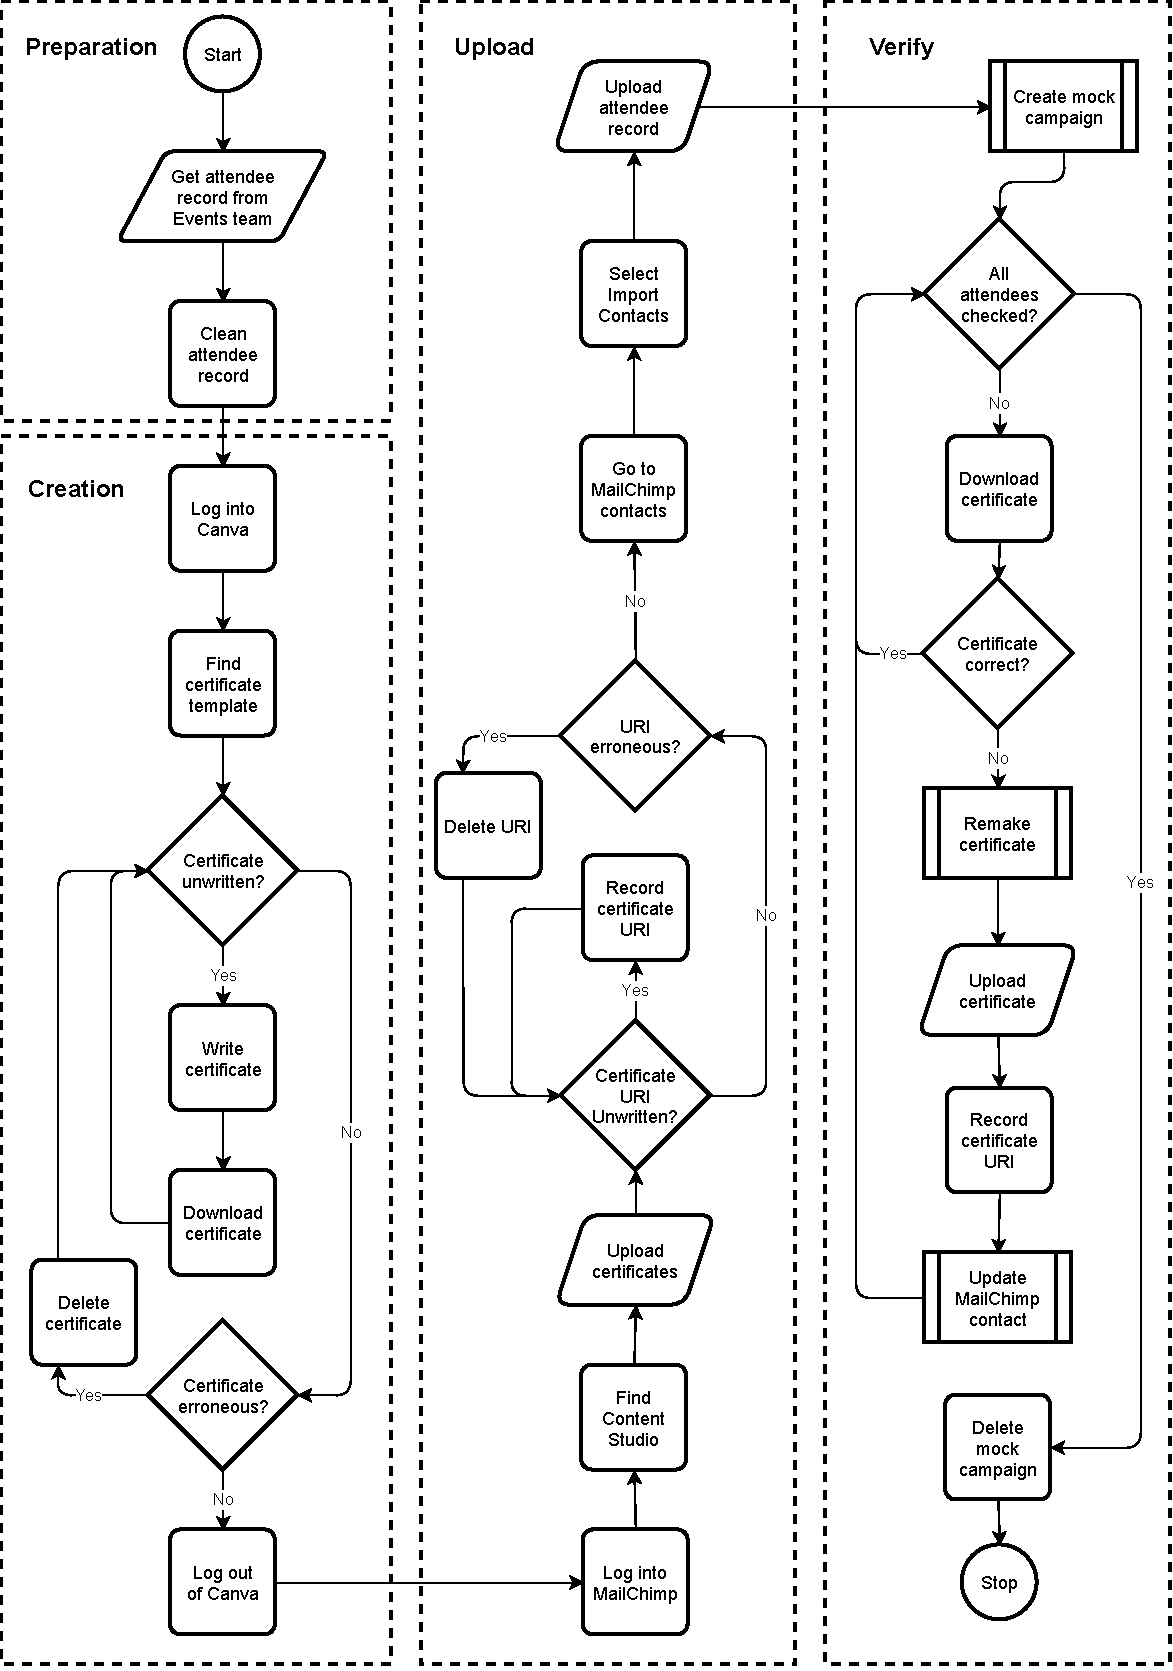
\includegraphics[width=\textwidth]{figures/old_solution.pdf}
    \caption{Old solution flowchart.}
    \label{fig:old-solution}
\end{figure}

\newpage

\section{Solution Overview}

\subsection{Rundown}

After some research, it has been discovered that stages 2, 3, and 4 of the old solution can be automated. For stage 1, instead of creating each certificate manually via Canva, the template can be created once and used to automatically create every certificate. Note that the template must be a Word document with merge fields or variables, not a PDF. The MailChimp API can be used to automate stage 3, where each certificate can be uploaded and have its URI recorded \cite{mailchimp-first-api-call}. With the URIs known, the attendee record can be updated and uploaded to MailChimp. Since the certificates were created automatically, stage 4 becomes redundant. This process is summarised in figure \ref{fig:new-solution}. With such a script, CIET can be confident in its ability to deliver the correct certificates to its members on time with minimal effort.

\begin{figure}[b!]
    \centering
    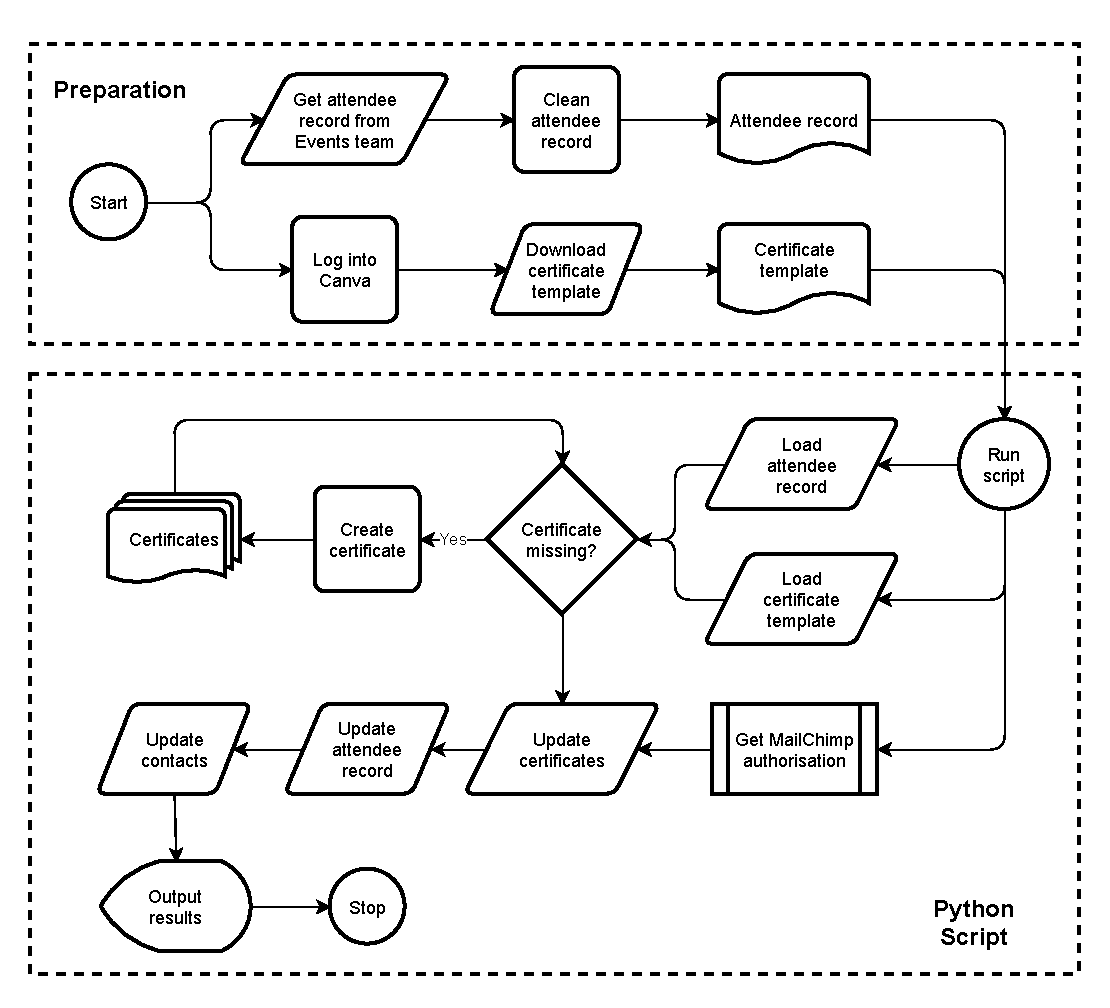
\includegraphics[width=0.8\textwidth]{figures/new_solution.pdf}
    \caption{New solution flowchart.}
    \label{fig:new-solution}
\end{figure}

Realising this goal, however, will require a well organised team and a plan. Due to the varied actions this script must perform, a moderately large codebase utilising several libraries is needed, demanding a significant time investment and expertise. This complexity is compounded by delegating the workload between a team, needing appropriate version control, task management, and enforeable coding standards. Furthermore, such a project could easily suffer from scope creep, especially with the user interface. Hence, the need for subsequent sections in this document.

\subsection{Proof of concept}

For the sake of time, a proof of concept can be implemented before scope creep becomes an issue. A proof of concept must include:

\begin{enumerate}
    \item Command line interface to run program.
    \item Must start program with certificate template path, attendee record path, and Mailchimp API and server keys as command line arguments
    \begin{enumerate}
        \item Strongly recommended to use \mintinline{python}{argparse} library.
    \end{enumerate}
    \item Must be able to load attendee records from a CSV file.
    \item Generate a certificate of attendance for each attendee.
    \begin{enumerate}
        \item Must be saved into a folder called \mintinline{shell}{/certificates} in the current working directory.
        \item Each certificate must be named based on attendee's full name.
    \end{enumerate}
    \item Upload certificates to Mailchimp, keeping track of the file URIs.
    \begin{enumerate}
        \item Uploading of certificates must be done as a batch, not individually uploaded.
    \end{enumerate}
    \item Update the attendee record with the certificate URIs.
    \item Update the Mailchimp contacts with file URIs.
    \item Inform the user of what the program is currently doing.
    \begin{enumerate}
        \item Can just be a simple sentence, e.g. "Uploading certificates to Mailchimp..."
    \end{enumerate}
    \item Be able to process errors without crashing.
    \item Must be able to continue processing certificates when one fails.
    \item Must inform user of which step or certificates failed and why.
    \begin{enumerate}
        \item Can be done once the program has finished everything else.
    \end{enumerate}
    \item All public and protected classes, methods, and function must have Google style docstrings \cite{google-docstring}.
    \item Must be able to run on Windows, Linux, and Mac systems capable of running Python 3.
\end{enumerate}

\noindent
For the sake of time and simplicity, the following assumptions can be made:

\begin{enumerate}
    \item The certificate of attendance is known.
    \begin{enumerate}
        \item The only field to be changed is the attendee name.
        \item The exact location of the attendee name field is known and constant.
        \item The merge field or variable of the attendee name field is known and constant.
        \item The certificate is always valid.
    \end{enumerate}
    \item The attendee record contains no errors.
\end{enumerate}

\subsection{Minimal Viable Product}

Once a proof of concept is complete, a minimal viable product (MVP) can be written. The MVP has all the criteria of the prototype, excluding 2, and

\begin{enumerate}
    \item Can be run via an executable or in the browser as a webapp.
    \begin{enumerate}
        \item No command line interfacing should be necessary.
    \end{enumerate}
    \item Should have a simple and initiative GUI.
    \begin{enumerate}
        \item GUI does not need to be aesthetically pleasing.
    \end{enumerate}
    \item Can select input files via file explorer.
    \item Must log at least info, warning, error, and critical messages to a log file.
    \begin{enumerate}
        \item Debug messages are optional.
        \item It must be known where the log file is.
        \item The GUI should have a button for viewing or downloading the log file.
        \item Strongly recommended to use the \mintinline{python}{logging} library.
    \end{enumerate}
    \item Must use OAuth 2 to get Mailchimp authorisation.
    \begin{enumerate}
        \item The program should not have the option to use API keys.
    \end{enumerate}
    \item Should be able to inform the user of errors that occur in real time without interrupting background tasks.
    \item Use appropriate colour coding and symbols to inform user of successes, warnings, and errors.
    \item Must be able to instantly respond to user inputs without stuttering.
    \item Multiprocessing and multithreading must be used to prevent the program from locking.
    \item Must be able to check attendee record for errors.
    \begin{enumerate}
        \item Repeated email addresses.
        \item Missing names or emails.
        \item Missing required fields.
    \end{enumerate}
    \item Must be able to display and select merge fields or variables in certificate template.
    \begin{enumerate}
        \item Must be able to view template within GUI.
        \item Must be able to select the merge field or variable where the full name goes.
    \end{enumerate}
    \item All code declared as public must be documented using Sphinx.
\end{enumerate}

\subsection{Competitive Product}

If the MVP is done, a competitive, market ready, version can be done. This version should have everything the MVP has and

\begin{enumerate}
    \item Must be able to load attendee records from an Excel file.
    \item Has ultra-specific error messages.
    \begin{enumerate}
        \item Informs the user of what exactly went wrong.
        \item Where possible, offers a solution.
        \item Where possible, offers links to online documentation.
    \end{enumerate}
    \item Must include install wizard with a build machine if not a webapp.
    \begin{enumerate}
        \item Must be able to choose where to install program.
    \end{enumerate}
    \item Allows user to select where log files are saved.
    \item Allows user to select what types of messages get logged.
    \item Must be able to select multiple fields in template as placeholders.
    \begin{enumerate}
        \item Must be able to select what each placeholder gets replaced with graphically.
        \item Must be able to select between attendee attribute, constant value (e.g. event name), or system value (e.g. timestamp).
    \end{enumerate}
    \item Must be able to generate PDF report of what happened.
    \begin{enumerate}
        \item Can select where report gets saved to.
        \item Can select what goes on the report.
    \end{enumerate}
    \item Must have an aesthetically pleasing GUI.
    \item Must have tutorials on how to use software.
    \item Must have a "Help" feature.
\end{enumerate}

\newpage

\section{Prerequisite Knowledge}

\subsection{Python Language}

While Python was originally designed as a simple scripting language, it has since evolved into one of the most used and popular languages. The simplicity of Python lends itself well to rapid prototyping, so simple that Python's syntax is often considered to be pseudocode. Furthermore, the library support for Python, both first and third-party, makes it extremely easy to make complex tasks simple. The sheer abundance of libaries available creates a compunding effect, as existing libraries makes it easier to wrote other libraries, leading to an exponential growth in library support. Whenever a new protocol or standard becomes prominent, chances are someone has already made a Python library to make it trivial to implement the protocol or standard within other programs. Additionally, the popularity of Python means there is ambundant support online for both known issues and asking online for assistance. For the sake of prototyping, it is difficult to find a better language than Python.

Considering the ambundance of support for Python, learning the language is best done with interactive tutorials found online. Such examples include W3 Schools \cite{w3-schools-python}, Codecademny \cite{codecademy-python}, and Learn Python \cite{learn-python}. Numerous other tutorials exist, such as those on Tutorials Point \cite{tutorialspoint-python} and the countless YouTube videos; however, these tutorials lack an interactive component, leading to reading or watching without learning. When learning a new language, the resource is less important than the interaction between the material and the student.

Where Python's weakness lies is in its performance. Since Python is a weak typed language, datatype checking must be done during runtime, greatly reducing performance. Far worse, the interpreted nature of Python means compiler optimisations cannot be performed, slowing down Python to a crawl. Compared to optimised compiled languages, such as C, Rust, and C++, Python performs dozens of times worse when comparing equivelant programs. This can be greatly mitigated by taking advantage of scientific libraries, such as NumPy \cite{numpy} and Pandas \cite{pandas}. These libraries are written in C and C++, allowing for speeds within the ballpark of C, C++, and Rust. However, certain conventions must be followed to take advantage of vectorised data, leading to data needing to be structured in vectors or matrices. Unfortunately, this will only result in a performance increase when doing mathematical operations on numeric data, such as vector dot products or summing an array. Ergo, Python is a poor choice for performance critical applications.

\subsection{HTTP Requests and Responses}    \label{sec:http}

Of interest to interfacing with internet-based servers is the hypertext transfer protocol (HTTP). Invented circa 1990, HTTP is a request-response protocol, transferring data in simple text documents. As of the time of writing, HTTP 1.1 is the most commonly used version, with 2.0 slowly replacing 1.1. In all versions, the first step is for the client to connect to the server via a TCP handshake. Once a connection has been established, the client can proceed to send a ``request'', which the server processes then replies with a ``response'' \cite{http-message}.

The request is a text document made of three, sometimes four parts. The first line is always the request header, formatted as the method type, followed by the path to the resource, then the HTTP version \cite{http-message}. Afterwards, each line then comprises the one key-value pair of the header, used to specify metadata, such as the host, accepted languages, authorisation codes, connection type, and expected content type(s) \cite{http-message}. To end the header, an empty line must then follow. For some requests, a body may also be necessary, such as the content being uploaded to the server \cite{http-message}. Below is an example of such a request.

\vspace{0.5\baselineskip}

\inputminted[linenos=true]{html}{http_examples/post_request.html}

Once the server has finished processing the request, it sends back a response, formatted very similarly to a request. The response's first line is always the status line, formatted as the HTTP version, the status code, then the status message \cite{http-response}. The status code is a three digit code informing the client of how the server handled the request. The first digit is the broad type of code, then the next two digits specifies the exact type of code. The status message is simply a humanly readable message version of the status code. After the status line, the header fields are then declared line-by-line, ending with an empty line. For some requests, a body will also be included after the empty line. See the example below.

\vspace{0.5\baselineskip}

\inputminted[linenos=true]{html}{http_examples/get_response.html}

\begin{info}[HTTP Status Codes]
For long messages split into multiple requests, a \texttt{1xx} status code means the server successfully received the segment and the client should send the next. \texttt{2xx} means the message was received, understood, and processed successfully. \texttt{3xx} means the server does not have the resource being requested but does know another server that does.\footnote{Responses with status codes of \texttt{3xx} should always include the server connection details in the body} 4xx means the client did something wrong, such as the classic \texttt{404} page not found error. Lastly, \texttt{5xx} means the server did something wrong.
\end{info}

As of HTTP 1.1, there are nine accepted methods \cite{http-methods}. Introduced in HTTP 0.9 (the first public version), the \texttt{GET} request is a simple read only request to retrieve a copy of a resource from the server \cite{http-0-9}. As of HTTP 1.0, the \texttt{POST} request allows for clients to upload new resources onto the server. Also as of HTTP 1.0, the \texttt{HEAD} request works identically to a \texttt{GET} request, expect that the body is not included. In HTTP 1.1, two important methods were added: A \texttt{PUT} request allows a client to replace an existing resource on a server with the one in the request body, whereas a \texttt{DELETE} request simply tells the server to delete the specified resource. Similar to a \texttt{PUT} request, a \texttt{PATCH} request tells the server to partially update a resource instead of replacing it. While not commonly used, HTTP 1.1 also introduced the \texttt{TRACE} and \texttt{OPTIONS} request types. The former performs a message loop-back test from the path of the specified resource, whereas the latter requests the server to describe all available commincation options for the specified resource. Lastly, the \texttt{CONNECT} request allows clients to connect to a server through another server, useful for setting up proxy servers or websites using TSL (i.e. HTTPS).

While HTTP 1.1 remains the predominant version as of the time of writing, HTTP 2.0 will eventually replace it. HTTP 1.1 introduced vast performance improvements over 1.0, most notably the ability to remain connected to the server after each request-response cycle instead of having to reconnect to the server. However, in 1.1, the server can only process one request from any client at a time, meaning the client must wait until the current request has been responded before sending another. This has changed in 2.0, allowing for mutliple requests to be sent, processed, and responded to after a connection has been established \cite{http2}, shown in figure \ref{fig:http-visualised}. For now, this project can ignore HTTP 2.0, but future versions may need to consider the inevitable obsoletion of HTTP 1.1.

\begin{figure}[h!]
    \centering
    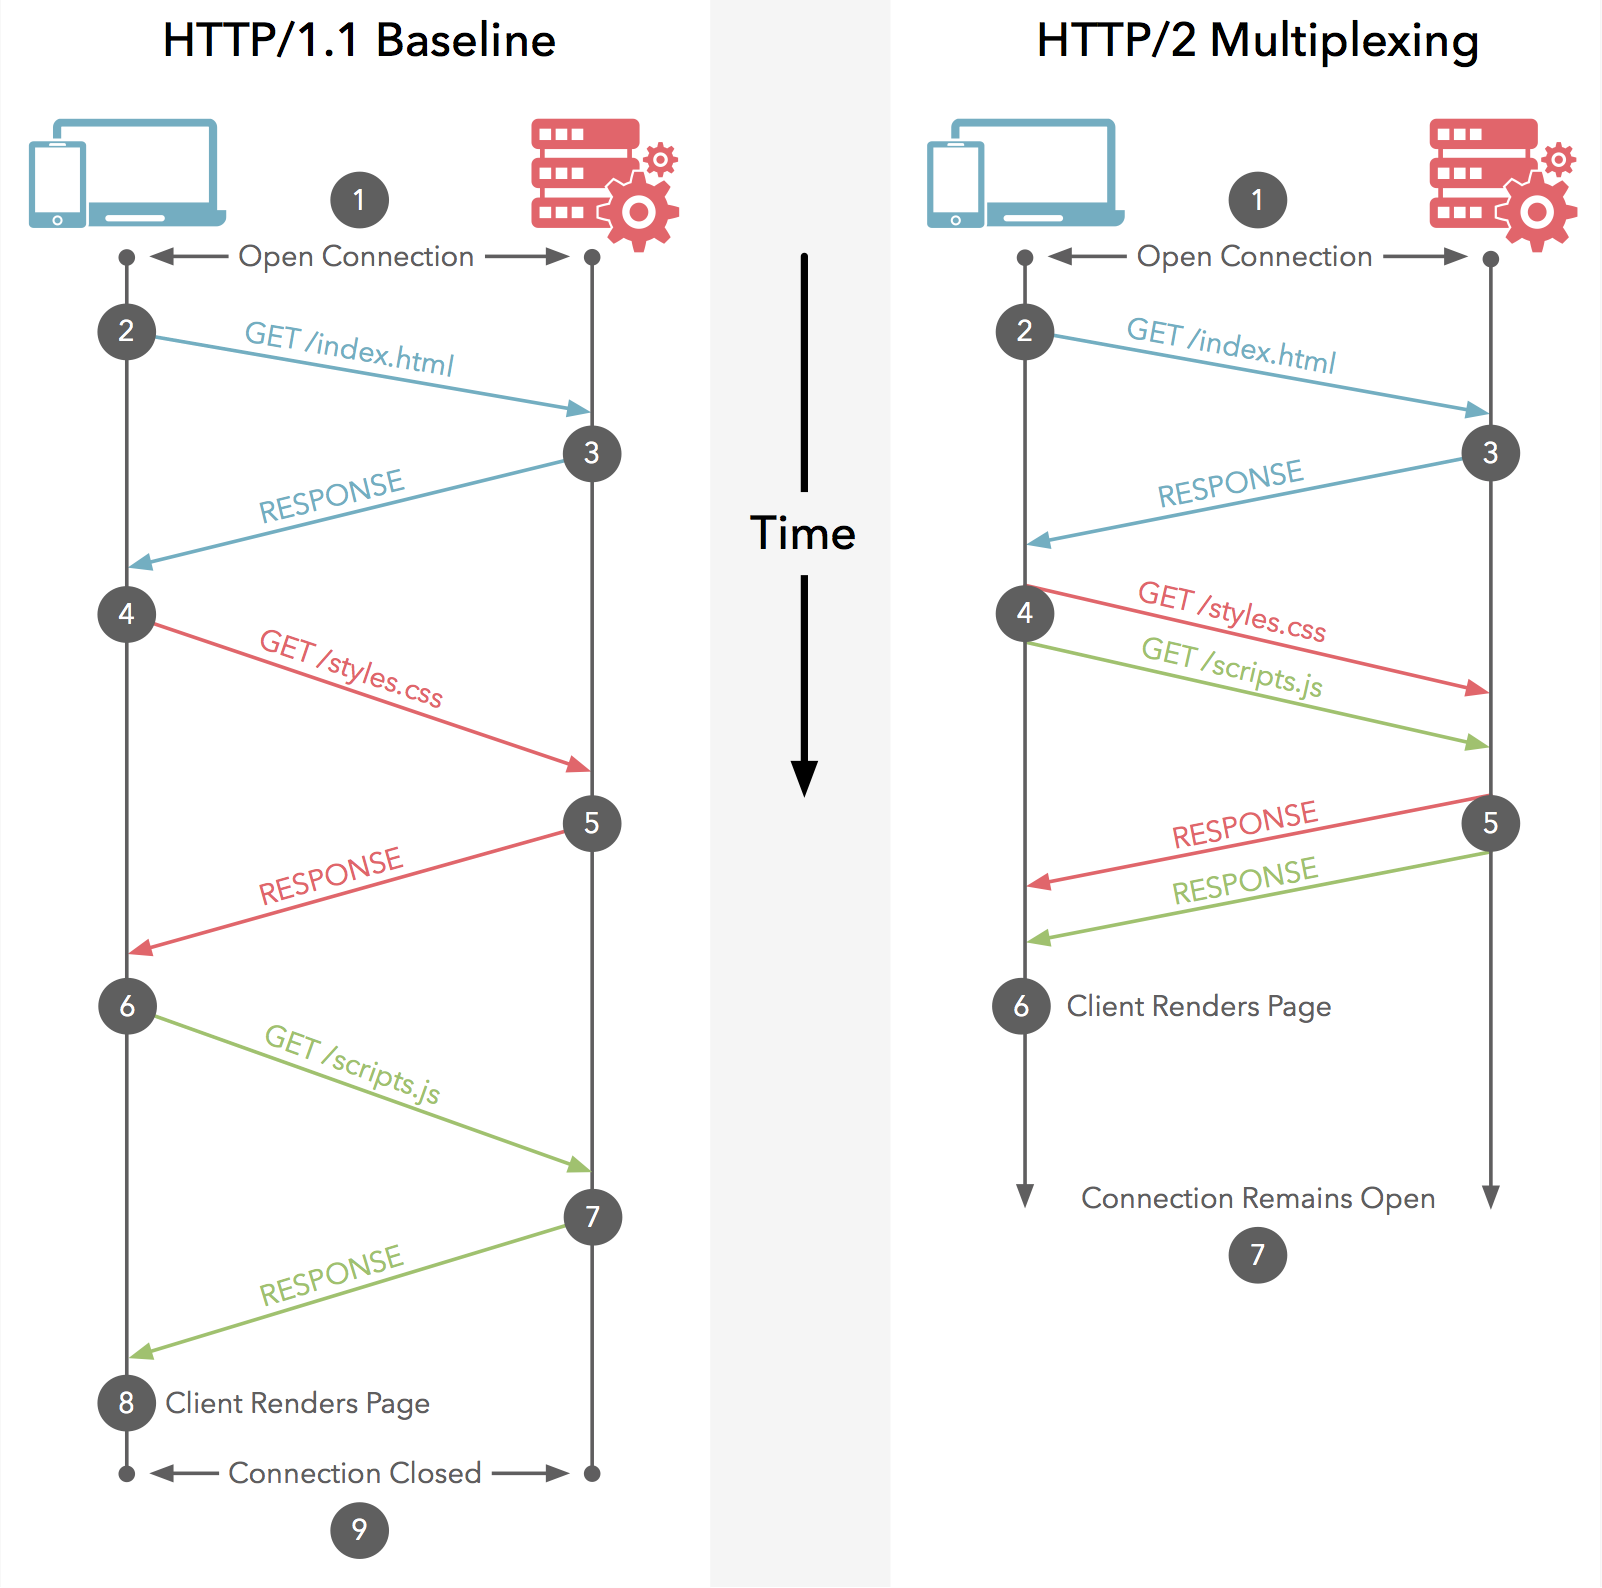
\includegraphics[width=0.9\textwidth]{figures/http1-vs-http2-multiplexing.png}
    \caption{HTTP 1.1 and HTTP 2.0 visualised \cite{http1-vs-http2}.}
    \label{fig:http-visualised}
\end{figure}

\subsection{Object Orientation}

Critical to software engineering, object orientated programming (OOP) has proven invaluable to large scale and collaborative code-based projects. This is possible via a sophisticated application of the broad divide and conquer approach, splitting complex programs into simple and decoupled modules and submodules. OOP achieves this through four main principles: encapsulation, abstraction, inheritance, and polymorphism.

\subsubsection{Encapsulation}

Consider the logistics in running a store: the stock available, the stock reserved for customers yet to buy them, preorders, cancellations, the stock on its way, the customers who have signed up as members, newsletters, purchases, overhead costs, etc. How does a business maintain such logistics? Who records the data? Who files and organises the data? Who has access to what data? Who is authorised to fix errors in the data and what process must they go through to make these fixes? Perhaps most importantly, who or what ensures the data is valid \textit{before} it is placed with existing data? Such problems can be at least mitigated using the OOP paradigm.

Since objects contain data as variables, the objects can be made responsible for protecting the data from corruption. Instead of making the variables directly accessible, the object can have getters and setters (also known as mutators) to access the data. Getters should always return a copy of the variable, whereas setters must validate the new value before setting the variable. For example, it is impossible for a jar to have a negative number of marbles, hence if outside code attempts to remove more marbles from a jar object than what is available an error can be raised and the jar's number of marbles remains unchanged. Similarly, the jar will probably also have a capacity, so that if too many marbles are attempted to be inserted a different error should be raised. Some object variable may not even have getters, such as the length of a collection (e.g. an array or a linked list). Instead, the length variable should automatically change as elements are inserted or removed. Even further encapsulated, other variables may not even have getters, as they may be variables that should only be used by the object internally, such as an array inside of a hash table. Protecting data like this greatly mitigates the data from being curropted or otherwise useless.

\begin{figure}[b!]
    \centering
    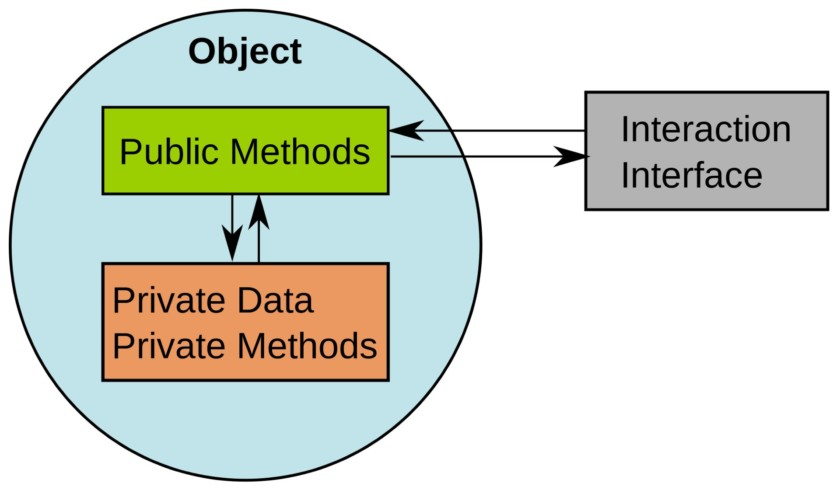
\includegraphics[width=0.5\textwidth]{figures/encapsulation.jpg}
    \caption{Encapsulation visualisation \cite{oop-encapsulation}.}
    \label{fig:encapsulation}
\end{figure}

In Python, encapsulation is implemented very differently to other OOP languages. Languages like Java, C\#, and C++ have the keywords \mintinline{c++}{public}, \mintinline{c++}{protected}, and \mintinline{c++}{private} for deciding how hidden a variable or method is. \mintinline{c++}{public} simply means anything that has access to the class or object can access the member, be it a variable or method. \mintinline{c++}{private}, however, means only the class or object can access the member, completely hiding it from all other code. While useful for data proctection, it was quickly found that \mintinline{c++}{private} is too restrictive for many applications. Instead, \mintinline{c++}{protected} has replaced \mintinline{c++}{private}, as it allows subclasses to access the member, dicussed further in the Inheritance subsection below. Python does not have these keywords, instead opting for using underscores: no underscores delcares the member (or ``attribute'' as it is known in Python) as public, a single underscore means protected, and a double underscore, or ``dunder'', means private. Protected and private variables can then be read using the \mintinline{python}{@property} decorator and set using the \mintinline{python}{@x.setter} decorator, where \mintinline{python}{x} is the variable being set. Note the example below and the lack of dunders.

\inputminted[linenos=true]{python}{python_examples/encapsulation.py}

\subsubsection{Abstraction}

As a program become more and more complex, it becomes increasingly difficult to manage the functionality of the program. Trying to track where the functions of a program are organised and located turns inpractical. Even trying to determine if a function has been implemented becomes time consuming and infeasible. This can be partially mitigated by organising functions into thematically narrow and consistent libraries; however, even this approach leads to too many functions to keep track of what has and has not been implemented. For complex programs, especailly those requiring extensive interaction with other programs, a smarter approach is needed.

Abstraction attempts to solve this issue by hiding functionality within objects. Abstraction is simply the process of hiding the implementation by only exposing what the object can do. Hence, outside code only needs to concern itself with what the object can do and not how it does it. Since objects can contain other objects, complex tasks involving several steps using numerous variables can be split accross a tree-like hierarchy of objects. Consider the complexity of sending and receiving HTTP requests and responses detailed in section \ref{sec:http}: with OOP all that is needed is a single \texttt{NetworkManager} that handles how an application sends and receives data without code outside the \texttt{NetworkManager} needing to know about how HTTP responses and request work. Therefore, outside code only needs to call a single method of one object and let it handle how the task is completed.

\subsubsection{Inheritance}

When similar entities need to be modelled, code repitition becomes an issue. Consider a pet tracker for a vetenary that needs to store various types of pets. Obviously, snakes and rabbits are two very different animals that require very different code to model. However, cats and dogs are similar enough that the code modelling these pets would at least somewhat repeat. Repeated code makes it more difficult to maintain, as each repeat must be individually tested, debugged, and modified due to changing environments or requirements, leading to the risk of some repeats not being debugged or changed properly. By extension, this also makes testing more expensive, time-consuming, and error-prone, as each repeat code block being tested will lead to repeat test cases. Clearly, such repitition needs to be eliminated.

\begin{figure}[b!]
    \centering
    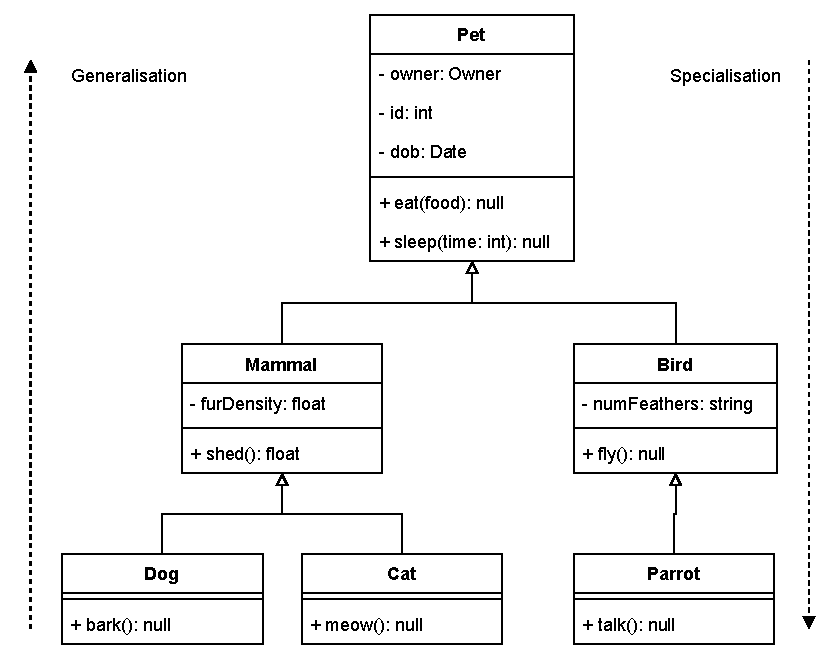
\includegraphics[width=0.7\textwidth]{figures/inheritance.pdf}
    \caption{Inheritance UML example.}
    \label{fig:inheritance-uml}
\end{figure}

OOP programming provides such a solution in the form of inheritance. Simply put, inheritance is the ability of some classes to inherit the code of other classes. For the pet tracker example, a base class called \texttt{Pet} or \texttt{Animal} can be made that contains code common to all pets. E.g., values like owner, pet ID, and date of birth. Further classes can be written that eliminate code repitition for groups of types of pets, e.g. \texttt{Mammal}, \texttt{Reptilian}, \texttt{Bird}, and \texttt{Amphibian}, each of which should inherit from the \texttt{Pet} base class. Then, more specific pet types can be written that inherit from these broad pet types, such as \texttt{Dog}, \texttt{Cat}, \texttt{Turtle}, \texttt{Snake}, \texttt{Parrot}, and \texttt{Frog}. Such inheritance is known as the \textit{is-a} relationship, as a dog \textit{is a} Mammal, which \textit{is a} animal. Designing a codebase like this completely eliminates repetitive functions, greatly speading up the process of writing the codebase and simplifying test cases.

Additionally, inheritance also covers one object being contained within another. This type of relationship is known as the \textit{has-a} relationship or association. For example, a car is \textit{not} a type of steering wheel and vice-versa. However, a car \textit{has a} steering wheel. Consider a car manufacturer that needs to design and manufacture cars. While different car models are not identical, they may share identical parts, such as a steering wheel. Hence, these identicial parts can be written, tested, and debugged once, then shared across the different car classes. This type of association is known as composition, as the car fully owns the parts it is made of. If the car object is destroyed, the car parts are also destroyed. This is opposed to aggregation, in which the child object can exist independently of the parent class, such as the cars and the manufacturer. As with the \textit{is-a} relationship, association greatly reduces code repitition.

\begin{wrapfigure}{r}{0.5\textwidth}
    \vspace{0pt}
    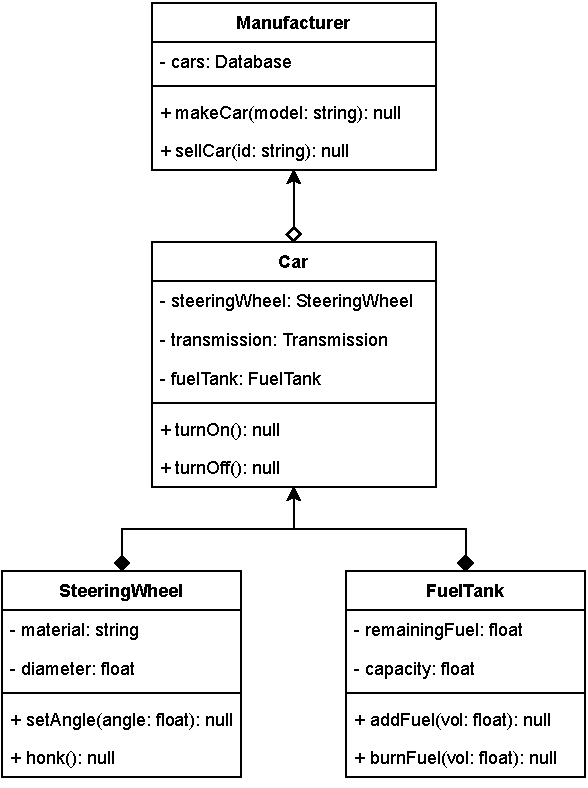
\includegraphics[width=0.48\textwidth]{figures/association.pdf}
    \captionof{figure}{Assocation UML example.}
    \label{fig:association-uml}
\end{wrapfigure}

\subsubsection{Polymorphism}

When developing a codebase, it occansionally becomes useful to have multiple functions or methods that are named the same but perform differently. In \texttt{C}, the \mintinline{c}{math.h} library contains functions for finding the absolute value of a number. There are actually two of these functions: the \mintinline{c}{abs()} function and the \mintinline{c}{fabs()} function. The reasoning being is that \mintinline{c}{abs()} takes in an integer whereas \mintinline{c}{fabs()} takes in a double. Since \texttt{C} is a strong typed language with no polymorphism, this practice of having multiple functions perform essentially the same task becomes inevitable. Even more complicated, consider the case of calculating the area of a shape. Since the areas of shapes are calculated differently from shape to shape, in \texttt{C} there would be one function per type of shape. E.g. \mintinline{c}{circleArea()}, \mintinline{c}{rectArea()}, \mintinline{c}{triangleArea()}, etc. As program requirements start involving extremely similar functions and datatypes, the number of near-identical functions to keep track of becomes inpractical.

Polymorphism solves this issue by allowing multiple functions to share the same name. One such manner of doing so is called ``method overloading'': allowing for a class or object to have multiple methods with the same name but different parameter lists in terms of their datatypes. In Python, this is actually not possible since the datatypes of variables does not have to be declared. Instead, Python achieves pseudo-overloading by allowing for a parameter to have one of multiple valid datatypes (such as \texttt{num} being either an \mintinline{python}{int} or an \mintinline{python}{float}) or by having parameters with default values. Further still, a function in Python can have an optional list of miscellaneous, unnamed parameters and another optional dictionary of named parameters. For example, the Python function

\begin{minted}{python}
def formatNumbers(num, *args, precision=2, **kwargs):
    ...
\end{minted}

\noindent
must be called with a number, but can allow multiple arbitrary numbers to be formated via the \mintinline{python}{*args} list, optionally specify the precision to format the numbers to (defaults to 2 decimal places), and also be called with arbitrary named parameters that are stored inside the \mintinline{python}{**kwargs} dictionary (short for ``keyword arguments'').

Using the \textit{is-a} inheritance principle, it is also possible to achieve polymorphism via ``method overriding''. Going back to the area of shapes example, we can calculate the areas of different shapes without needing multiple methods with different names. Instead, a base class \mintinline{python}{Shape} can be written, that has the method \mintinline{python}{calcArea()}. This method is known as an ``abstract method'' since it has not been implemented, meaning the \mintinline{python}{Shape} class is also abstract. Abstract classes cannot be instantiated into objects, making them useless by themselves. Instead, subclasses of the \mintinline{python}{Shape} class can be written that implement this abstract method, such as \mintinline{python}{Circle}, \mintinline{python}{Rectangle}, and \mintinline{python}{Triangle}. The significance of which means that outside code does not need to concern itself with what exact type of shape a \mintinline{python}{Shape} object is, only that is has a \mintinline{python}{calcArea()} method. Hence, functions can be written once for any arbitrary shape object and more shape types can be written latter without having to change any of these functions.

\subsection{Application Programming Interface}

The world of modern software development is one heavily comprised of using code and services created by third-party organisations or individuals. This is an inevitable consequence of the daunting product requirements that modern software must abide by to remain competitive. However, the pitfalls of using third party services quickly become apparent: \textit{How do we know future changes won't break our code? Will our application still work when this service changes? What security flaws or exploits are exposed allowing others to use our service? What do we do if a third party service does not allow us to access their service via code?} Consider the need for a music editing mobile app that can use music owned by the user from their Spotify, Google Music, Bandcamp, or Apple Music accounts. How does a development team even begin to integrate these services their mobile app?

Solving these concerns introduces the need for Application Programming Interfaces, or APIs. An API, simply put, is a set of commands a program can use to access and upload data to another program. They can be as simple as the set of functions and constants within a library to the monolithic 2 billion line of code Google API \cite{google-api}. Well designed APIs allow external parties to develop their own applications integrating your service without needing to know how the API works, nor what the external application is or does. APIs also greatly mitigate security issues, as APIs can hide implementation or block access. External developers using an API can also be sure that future changes to the API will not break their application, as updates come with a version number, signifying if an API change has occurred. If an API change has occurred, the external developers can simply not use the newer version until they have updated their application to use the newer API. Most relevant to this project, the Mailchimp API is the only way a program can access a user's Mailchimp account without hacking the Mailchimp servers. Without this API, the project would not be possible.

\subsection{JSON}

While developers can use whatever common or obscure data format they want for their APIs, JavaScript Object Notation (JSON) has dominated API usage in recent years. Originally designed for the Javascript programming language as a way of creating objects without a class or constructor function, JSON has since evolved into a text format for storing and transporting data in a lightweight manner \cite{json}. While confusing for new comers, it quickly becomes evident as to why JSON is so popular: its ability to scale for various types of data easily in a humanly readable format.

JSON is comprised of a few special characters and a few datatypes. Most JSON message always starts and ends with curly brackets, denoting the message as an object \cite{json}. The properties of the object are then writtin in key-value pairs, where the key is always a string. The value can either be a string (within quotations), a number, an array (denoted using square brackets), a boolean (either \mintinline{json}{true} or \mintinline{json}{false}), \mintinline{json}{null}, or a nested object (denoted with curly brackets). The following JSON conventions are either required or strongly recommended:

\begin{enumerate}
    \item Key names must always be strings.
    \begin{enumerate}
        \item Key names should be alphabetical where possible.
        \item Key names should use hypens or (preferably) underscores instead of spaces.
        \item \texttt{snake\_case} is preferred over \texttt{camelCase} for key names.
    \end{enumerate}
    \item Whenever the elements in a collection have unique identifiers, they should be stored in a nested object.
    \item Whenever the elements in a collection do not have unique identifiers, they should be stored in an array.
    \item Whenever the elements in a collection need to be ordered, they should be stored in an array.
    \item Nested objects should contain data modelling a single entity.
    \item An array should contain elements of the same datatype.
    \item If an array stores objects, every object should have the same keys.
    \item Always use quotations ("") instead of quotes (`') when declaring a string.
    \item If a value is not known, assign it as \mintinline{json}{null}.
\end{enumerate}

Below is a simple example of a club's details stored in JSON format:

\inputminted[linenos=true]{json}{json_examples/club_details.json}

\newpage

\section{Attendee Management}

\subsection{Internal storage of attendees}

Each attendee will need to be stored as an object, requiring the ability to read and write both required and optional attendee attributes. At a minimum, the attendee objects will need to store the email address, given name, and family name. Furthermore, future upgrades may require other attributes to be stored. Since these optional attributes are not known, the attendee object must have methods for adding, getting, updating, and removing any arbitrary attributes. Fortunately, the attendee objects only need to store data, meaning no methods beyond setters and getters are needed.

Once the interface for an attendee class has been agreed upon, an attendee manager can be written. This attendee manager will store all attendee objects for convenience across all other modules that use the attendee records. Hence, the attendee manager will need methods for adding attendees, iterating over attendees, and removing attendees. Updating attendee records can be done via the attendee objects themselves, as they will already validate the data. Since the attendee objects already validate themselves, the attendee getters in the attendee manager should return a reference to the attendee, not a copy. This is to ensure that updating an attendee record can be done with removing and re-inserting the attendee. To keep track of each attendee within the manager, each attendee will need some unique identifier, which can be the email address.

\subsection{Attendee File IO}

Given that the attendees must be loaded and stored from a CSV file, an attendee file manager will be needed. Since the attendees are stored as tabular data, the Python Pandas library can be used to store the attendee data \cite{pandas}. It is important to note that this data is raw in nature, meaning it will not be validated beyond any file IO error checking. The purpose of the attendee file IO module is just to load the raw data in tabular form, needing further data validation from the attendee and attendee manager classes. Ergo, an iterator should be implemented to retrieve the raw attendee data one-by-one.

Once the attendee records have been internally finalised, they will then need to be saved to a file. Considering that the data is already in tabulated form, it should be a simple matter of saving the data in a CSV file.

\subsection{Further reading}

\begin{itemize}
    \item Python pandas: \url{https://pandas.pydata.org/}
    \item Python CSV module: \url{https://docs.python.org/3/library/csv.html}
\end{itemize}

\newpage

\section{Certificate Editing and Creation}

\subsection{Approach}

Once the attendees are known, the certificates can be made. Unfortunately, the certificate template on Canva is useless, as it cannot be downloaded as a editible document. Instead, the certificate template should be recreated in Word with at least one merge field or variable (denoted via double braces) for the attendee name. Word documents can then be loaded into Python with their merge fields or variables identified via the \texttt{docx-mailmerge} or \texttt{docxtpl} Python libraries. Once the attendee's details has been inserted, the certificate can be saved as a Word document then converted to a PDF via the \texttt{docx2pdf} library. With these libraries, all certificates can easily be created from a template.

\subsection{Further Reading}

\begin{itemize}
    \item \texttt{docx-mailmerge} library: \url{https://pypi.org/project/docx-mailmerge/}
    \item \texttt{docxtpl} library: \url{https://pypi.org/project/docxtpl/}
    \item \texttt{docx2pdf} library: \url{https://pypi.org/project/docx2pdf/}
\end{itemize}

\newpage

\section{MailChimp Authorisation}

To prevent malicious parties from accessing Mailchimp accounts, applications must provide authorisation with each HTTP request. The Mailchimp API provides developers two methods of auto-authorisation: an API key and OAuth2, both with their strengths and weaknesses.

\subsection{Using API and Server Keys}

Owners of a Mailchimp account can use their API and server keys to allow applications to access their account. The developer simply needs to log into their Mailchimp account, generate an API key, find the server key in the URL, then input both keys into their application \cite{mailchimp-api-key}. The power of API keys lies in their simplicity, only needing a few minutes to generate and start using the API key. Once the key has been retrieved, the key just needs to be included into the config of HTTP requests to Mailchimp, only taking a few lines of code \cite{mailchimp-first-api-call}. The example below is taken straight from the Mailchimp API:

\inputminted[linenos=true]{python}{mailchimp_examples/mailchimp_ping.py}

\noindent
If the request succeeds, the response body will contain

\inputminted{json}{mailchimp_examples/ping_response.json}

However, an API key is equivelant to a root admin's login details: giving full permissions to the entire account. With an API key, a developer can change user permissions, modify contacts, and send emails. For security reasons, all API keys can be disabled at any time, preventing compromised keys from being used negligently or maliciously \cite{mailchimp-api-key}. Regardless, it is extremely rare an app will need full access to a Mailchimp account.

Furthermore, asking a user to generate then input their API is a very user unfriendly task. First off, the average user will have no idea what an API even is, none-the-less an API key. Secondly, the user must ensure to never share or write down their API key outside of the app, which is extremely unlikely, causing a high security risk. Similarly, the app must be secure enough to not expose the API key, which is extremely difficult for a webapp. If an API key is exposed by a service provider, the provider must notify their users ASAP and the users must disable the API key before being hacked. Clearly, API keys present a high risk for applications, especially when accessing accounts not owned by the service provider.

\begin{warn}
Under no circumstances should an API key ever be disclosed to anyone! This includes any written form, even in source code! Authorised individuals should log into the associated account to get the API key. The API should not be written down, instead it should be an environmental variable on a secure device, where the application can access it. It should never be saved by the application to a file or sent anywhere outside the service requiring the API key!
\end{warn}

\subsection{Using OAuth2}

\begin{figure}[b!]
    \centering
    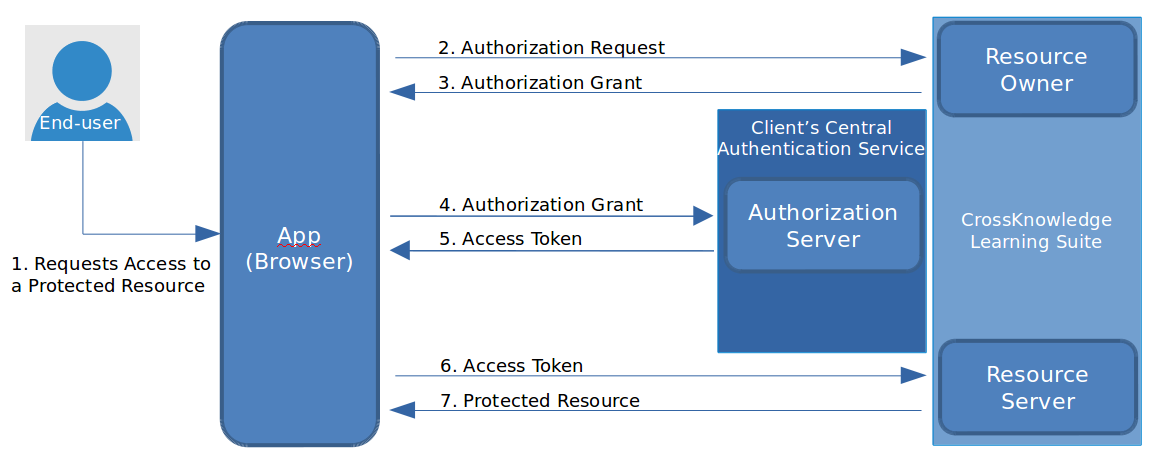
\includegraphics[width=\textwidth]{figures/oauth2workflow.png}
    \caption{OAuth2 simplified flowchart \cite{oauth2-fig}.}
    \label{fig:oauth-flowchart}
\end{figure}

A far more modern method of gaining access to a user account from another service is to use the OAuth2 protocol. Short for Open Authorization 2.0, OAuth2 has quickly become the de-facto way for electronic services from different organisations to communicate with each other automatically \cite{oauth2}. The protocol is comprised of several steps: first, the app must be registered on the service, which will provide a \texttt{client\_id} and \texttt{client\_secret}. Next, the app the user is running requests access from the user to another service. If the user agrees, the app makes an authorisation request to the third-party service using the \texttt{client\_id}, redirecting the user to login to the account they own. Once logged in, the service will ask the user to confirm that they consent to giving the displayed permissions to the app. If the user agrees, the user is then redirected back to the app, such that the app gets an authorisation code. The authorisation code and \texttt{client\_secret} can be exchanged for an access token (a long, computer generated hexadecimal string). With the token, the app can access the user's resources. Alternatively, an implicit grant skips a step by getting a token instead of a code to exchange a token. This is useful for situations where it is not possible to secure the \texttt{client\_secret} in the app (such as a Desktop or mobile app). Figure \ref{fig:oauth-flowchart} visualises this process.

While more complicated to implement than using an API key, OAuth2 has multiple key advantages. Firstly, the app requesting access never observes the login details for the service, as the service takes control when this happens. Next, the app only has access to what the user authorises, not the entire account. Additionally, tokens provided by the service expire quickly, usually after an hour. Ergo, if the token gets leaked, it will either expire soon or have already expired. Furthermore, if an app becomes comprised, all services which the developers registered their app on can have their app authroisation code disabled, preventing all authorisation requests. Lastly, it is far easier for a user to enter in their login details than provide an API key. Clearly, OAuth2 is a far more powerful and secure way of exchanging data between services or apps than API keys.

\subsection{Further Reading}

\begin{itemize}
    \item OAuth2 official documentation: \url{https://www.oauth.com/}
    \item OAuth2 and OpenID Connect explained: \url{https://www.youtube.com/watch?v=996OiexHze0&t=3326s}
    \item \texttt{python-oauth2} library: \url{https://pypi.org/project/python-oauth2/}
\end{itemize}

\newpage

\section{Certificate Uploading}

\subsection{Doing single POST requests}

After gaining Mailchimp authorisation, the certificates can be uploaded to Mailchimp. First of, a folder should be created to store the files within. According to the Mailchimp API, this is possible by making the POST request below \cite{mailchimp-add-folder}:

\inputminted[linenos=true]{python}{mailchimp_examples/create_folder.py}

\noindent
The response of which will contain the folder ID, an integer that uniquely identifies that folder. Given the folder ID, the certificates can then be uploaded via a the POST request \cite{mailchimp-add-file}

\inputminted[linenos=true]{python}{mailchimp_examples/upload_file.py}

\noindent
The responses of uploading the files will contain a \texttt{full\_size\_url} field, which is needed for the next section. Hence, a functional Mailchimp manager module will need a function to take in the certificates, the certificate filenames, and the folder name. Given these parameters, the folder must be created first, have its folder ID recorded, then upload the certificates into the folder. As the responses from uploading the certificates are received, the \texttt{full\_size\_url} must be recorded and returned to the caller.

\subsection{Doing multiple async requests with batches}

However, the exact manner in which the requests are made can cause the program to lock up for prolonged periods of time. This is due to the \mintinline{python}{client.fileManager.create_folder()} and \mintinline{python}{client.fileManager.upload()} functions being ``blocking functions''. Such functions halt the program's progress for a long period of time. In this case, it is caused by waiting for a response from the Mailchimp server. Furthermore, to prevent server overloading, the Mailchimp API will only allow 10 concurrent requests per API key \cite{mailchimp-batch}. Considering that it takes 120 seconds for the for a request to time out, the worst case scenario is that it will take an hour and 40 minutes to process 50 attendees in a sequential manner. With concurrent requests, this worst case reduces to 10 minutes, still far too long for a user to wait.

The solution is to use Mailchimp's batch feature. Instead of making one POST request per certificate, all the POST requests can be bundled into a batch \cite{mailchimp-batch}. Making the batch request given the individual requests is trivial, as the body of the request is simply a JSON object containing one field, \texttt{payload}, whose value is a Python list (or JavaScript array) of the individual requests. The code below is Mailchimp's example of adding 1000 contacts at once \cite{mailchimp-batch}.

\inputminted[linenos=true]{python}{mailchimp_examples/batch_request.py}

Furthermore, the \mintinline{python}{response = mailchimp.batches.start(payload)} is not a blocking function. Instead, it returns a response that Mailchimp generates and sends as soon as possible, even though the individual requests have not been processed \cite{mailchimp-batch}. The body of the initial request includes a batch ID, which can be used to do another request to see the status of the batch via

\mint[linenos=false, frame=none]{python}|response = mailchimp.batches.status(batch_id)|

\noindent
Once all requests have been processed, a gzipped archive of the responses can be downloaded through the \texttt{response\_body\_url} available in the batch response. 

Since downloading, extracting, and processing the responses would be slow, it is strongly recommended the method that makes the batch request simply return the final batch response. If the responses are desired, then another method should be written to use the \texttt{response\_body\_url} to download the responses. From there, the file can be unzipped, which reveals one JSON file per request. It should be noted that Mailchimp will only store the responses for seven days \cite{mailchimp-batch}. Furthermore, the \texttt{response\_body\_url} will only last for 10 minutes for security purposes. If the \texttt{response\_body\_url} expires, another can be retrieved via a batch status request using the batch ID.

\subsection{Using callbacks to retrieve the status}

Since it will take a noticable amount of time to process the requests, the user should be informed of how the request is going. However, when calling the method that does the batch request, control of the program is handed over to this method until the batch is complete. Hence, a callback will be needed to inform the user of the batch's progress. This callback should be called whenever the batch progress changes. Combined with multithreading, this will allow for a program that can simultaneously handle user inputs, output the current status of a batch request, and perform the batch request.

\subsection{Further reading}

\begin{itemize}
    \item Mailchimp API: \url{https://mailchimp.com/developer/marketing/}
    \item Mailchimp batch requests: \url{https://mailchimp.com/developer/marketing/guides/run-async-requests-batch-endpoint/}
    \item Mailchimp API limits: \url{https://mailchimp.com/developer/marketing/docs/fundamentals/#api-limits}
    \item Mailchimp file manager API: \url{https://mailchimp.com/developer/marketing/api/file-manager/}
\end{itemize}

\newpage

\section{Contact Updating}

Once the certificates have been uploaded with the file URIs recorded, the attendee list can finally be updated. This can be accomplished via a method in the attendee manager taking in a mapping between the attendees and their certificate URIs, then updating the attendee objects. Once updated, the attendee objects can be saved as a CSV file, overwriting the original attendee record. Lastly, the attendee CSV file can then be uploaded to Mailchimp via a batch request. However, care must be taken as some attendees may not be contacts on our Mailchimp account or existing contacts using a new email address.\footnote{Mailchimp uses the email address as the unique identifier, so existing members can be added multiple times through different email addresses. This has been an ongoing issue with our members for years.} The Mailchimp API provides a PUT request for adding or (if already exists) updating a contact, shown below \cite{mailchimp-update-member}. Once all contacts have been updated, the program can finish.

\inputminted[linenos=true]{python}{mailchimp_examples/add_or_update_member.py}

\subsection{Further reading}

\begin{itemize}
    \item Mailchimp members API: \url{https://mailchimp.com/developer/marketing/api/list-members/}
    \item Mailchimp API: \url{https://mailchimp.com/developer/marketing/}
    \item Mailchimp batch requests: \url{https://mailchimp.com/developer/marketing/guides/run-async-requests-batch-endpoint/}
    \item Mailchimp API limits: \url{https://mailchimp.com/developer/marketing/docs/fundamentals/#api-limits}
\end{itemize}

\newpage

\section{User Interface}

\subsection{Command Line Interface}

For the sake of a prototype, a command line interface (CLI) can be implemented. In Python, the simplest and fastest way of implementing a CLI is through \mintinline{python}{print()} function calls. While simple, the \mintinline{python}{print()} function is extremely limited. Most notably, the \mintinline{python}{print()} function does not allow for the text cursor to be moved backwards, meaning the entire screen must be cleared or enough lines must be written to remove old text. Additionally, the lack of colour coding heavily reduces readability, as successes, warnings, and errors are not immediately obvious. Additionally, displaying boxes and other structured displays is extremely tedious and inpractical with \mintinline{python}{print()}. While it is possible to achieve such feats in a terminal, different terminals use different codes for colour and special formatting, all of which are complex and highly difficult to read and understand. This leads to numerous compatibility issues between terminals.

Going back decades, the \texttt{curses} library attempts to partially mitigate the limitations of the humble \mintinline{python}{print()} function. Implemented in C, Python's \texttt{curses} library is simply a set of wrappers calling the C \mintinline{C}{ncurses.h} functions \cite{curses-python} \cite{ncurses}.\footnote{The ``n'' is short for new.} This alone has two advantages: (1) this makes it extremely easy to transition between C and Python when using \texttt{curses}, and (2) the functions are highly optimised. This is on top of the ability to easily colour text, move the cursor around, and draw boxes. While simple in concept, figure \ref{fig:ncurses-example} below is an example of advanced usage of the \texttt{curses} library. Using \texttt{curses}, it is possible to easily create GUI-like user interfaces without the complexity of GUI frameworks.

\begin{figure}[b!]
    \centering
    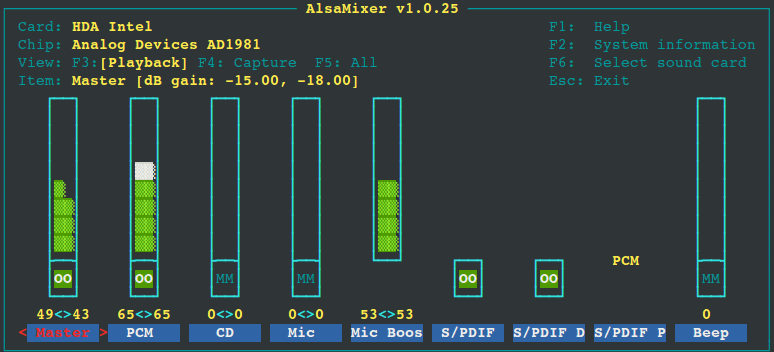
\includegraphics[width=\textwidth]{figures/ncurses_example.png}
    \caption{Advanced example of \texttt{curses} \cite{curses-api}.}
    \label{fig:ncurses-example}
\end{figure}

At a minimum, a CLI must meet certain criteria. For each stage the program is in (see figure \ref{fig:new-solution}), at least one line of text must be printed. For stages that involve processing a collection of items, the program should \textbf{not} print one line per item processed; it should update the line with a progress bar\footnote{See the \href{https://pypi.org/project/tqdm/}{tqdm} library} or a fraction \textit{without} clearing the screen. For any error that occur, the error should either be printed at the end of the program's life or printed immediately then force to the to confirm before continuing. Any inputs required from the user can either be done as command line arguments or the \mintinline{python}{input()} function. A example of such a CLI is shown below.

\inputminted[]{shell}{cli_examples/simple_cli.txt}

\subsection{Desktop GUI}

While useful for prototyping and developers, CLI have not been suitable for the average computer user for decades. Instead, graphical user interfaces (GUI) are the norm. Whereas CLIs are sequential, always following some order of IO actions in a linear of tree structure, GUIs are event driven. In GUIs, the structure of the interface remains constant until an event occurs, such as the user selecting a button, saying ``Hi, Siri'', or a message being received over the internet. GUIs achieve their event driven nature via heavy usage of callbacks and OOP: an object is given the callback, then sits and waits until an event or ``trigger'' occurs. Once the trigger activates, the object uses the callback to determine what to do. Separating the when (the object) from the what (the callback) allows for reusable and small code.

In Python, creating a GUI for a desktop application requires one of several GUI frameworks. These differ from Python wrappers around older frameworks, such as Qt5 and wxWdigets \cite{qt} \cite{wxwidgets}, to pure python, like TKinter and PySimpleGUI \cite{tkinter} \cite{pysimplegui}, and hybrid framworks, like Kivy \cite{kivy}. Most frameworks still in use have maintained relevance by finding a niche. The older frameworks implemented in C++ are well-established with online support and documentation going back decades, as well as being highly efficient, running extremely fast with minimal overhead. Newer GUI frameworks made for Python benefit from simpler APIs, encouraging faster development. Choosing a framework is a matter of the product requirements, both for current builds in development and future versions.

By far the most popular, so much so that the option for installing the framework is included when installing Python, is Tkinter. Well known for its simplicity and user friendly GUI builder, Tkinter tends to be a Python programmer's first GUI framework. While excellent for simple Python projects, Tkinter is restricted to Python, meaning the code and assets cannot be reused for other programming languages. This represents a fatal flaw when attempting to redo a codebase in a different language, as the GUI must be completely redone. Additionally, Tkinter being a Pythonic framework suffers from performance issues relative to older frameworks. Hence, Tkinter and similar Pythonic GUI frameworks are inappropriate for this project.

Kevi is a more interesting GUI framework based on its specialty. Kevi is written Cython, making it a Pythonic framework, implying it is incompatible with other languages. Where Kevi excels is mobile app development, as its widgets are designed with touchscreens in mind and the native assets of desktop applications are ignored. This makes rapid development of mobile apps feasible once the small learning curve has been overcome. Hence, for purely Python projects with mobile development in mind, Kivy is a good choice.

Out of the older GUI frameworks, only Qt and wxWdigets have remained competitive. Fortunately, both Qt and wxWdigets have Python wrappers, called PyQt and wxPython \cite{pyqt} \cite{wxpython}. Both are fast and efficient frameworks with multithreading and multiprocessing built-in, with wxWidgets being slightly faster due to its simpler design. Additionally, wxWidgets has a lower learning curve with only just above 20 widgets available. The con, however, means that wxWidgets is not as powerful as Qt. Despite Qt's far higher learning curve, Qt Designer allows developers to quickly design a GUI without writing a single line of code. Even better, Qt Designer exports GUIs to \texttt{.ui} files, compatible with Qt across all languages without modification. Hence, Qt is favourable over wxWidgets for the more complex product requirements.

Clearly, all these GUI frameworks have their pros and cons. Choosing one should be primarily a matter of which one fits the program requirements the best.

\subsection{Webapp}

With the rise of high-speed internet, most developers have moved away from installable desktop applications and embraced web apps in their place. The benefits of which are immediately obvious: the app can be used without installation of any software, the user's OS is abtracted through the browser, and most of the code and assets used to create the app can be hidden on servers. From a user's perspective, it is simply far more convenient to use an app immediately instead of waiting for a download to finish, installing the software (taking potentailly valuable storage space), then have to worry about compatibility issues with their device. A constant internet connection also guarantees updates and announcements can be made immediately, instead of annoying the end-user with ``Update available'' notifications. Furthermore, advancements in public clouds, such as Microsoft Azure, Amazon Web Services, and Google Cloud, have made it far more seemless for developers to build webapps without needing to build nor maintain private servers. Lastly, the internet connection allows for mass data collection of user behaviours and activities, vital to further app improvements and marketing. From these advantages, it is clear as to why modern developers have made the switch to webapps.

This flexibility, ease of use, and scalability comes at a cost: the constant maintenance required, cybersecurity concerns, and server costs. This is in addition to the setup required, needing a front-end UI, backend databases, an administrator control view, an auditing system, interfaces for third-party services, among numerous other systems. Typically, these systems are built using various programming languages, requiring expert knowledge in numerous protocols. While a for-profit business may be able to afford such costs with full time staff, a student club would struggle to find the finances and people to build and maintain such a system.

\subsection{Further reading}

\begin{itemize}
    \item Python \texttt{curses} library: \url{https://docs.python.org/3/howto/curses.html}
    \item Tkinter documentation: \url{https://docs.python.org/3/library/tkinter.html}
    \item PySimpleGUI: \url{https://pysimplegui.readthedocs.io/en/latest/}
    \item Kivy website: \url{https://kivy.org/#home}
    \item Qt website: \url{https://www.qt.io/}
    \item Qt designer download: \url{https://build-system.fman.io/qt-designer-download}
    \item \texttt{PyQt} documetation: \url{https://wiki.python.org/moin/PyQt}
    \item wxWdigets website: \url{https://www.wxwidgets.org/}
    \item wxPython website: \url{https://wxpython.org/}
\end{itemize}

\newpage

\section{Version Control}

\subsection{Context}

Pre-2002, the Linux OS was extremely difficult to maintain due to its open-source nature. Changes were passed around as patches and archived files, all of which assumed specific versions of the Linux OS were already installed \cite{git-short-history}. As Linux grew into numerous distributions, all of which had their own developers with their own patches, it became extremely difficult to keep track of what patches needed to be installed. Even worse, the complexity of the patches grow exponentially as distributions split off into multiple distributions. Sometimes, a user should install a patch as it affected the Linux Kernel or the exact distribution installed, whereas other times installing a patch could break the user's system. This is assuming the user can even find the patches to begin with, a task that can prove frustrating and time consuming in of itself.

To better manage the various Linux distributions and their respective patches, BitMover, a for-profit business, allowed the Linux team to use their version control software (VCS) BitKeeper for free \cite{git-short-history}. The condition being that Linux developers were not allowed to develop software that competes with BitMover's products. The relationship was uneasy, as many of the pro-open software Linux developers were not happy with using a commercial service by a for-profit business. In 2005, the relationship between the Linux team and BitMover broke down when a developer added commercial features for free. With no VCS to use, the Linux team needed a replacement.

\subsection{What is Git?}

The replacement came in the form of the open-source software Git. Designed to be lightweight, fast, and simple to use, Git has become the dominant VCS software worldwide. In short, Git allows a team of developers to collaboratively work on a project without the hassles of conflicting code changes, file reserving, nor untracked changes. This is achieved through a tree based version control structure, where each new feature, bug fix, or documentation update is tracked in its own branch of the tree. Within each branch are ``commits'': snapshots of the tracked files with a short description of what changed and why. Once the update is complete, the branch can be ``merged'' back into the master (or main) branch. Figure \ref{fig:git-basic-usage} visualises such a workflow.

\begin{figure}[t!]
    \centering
    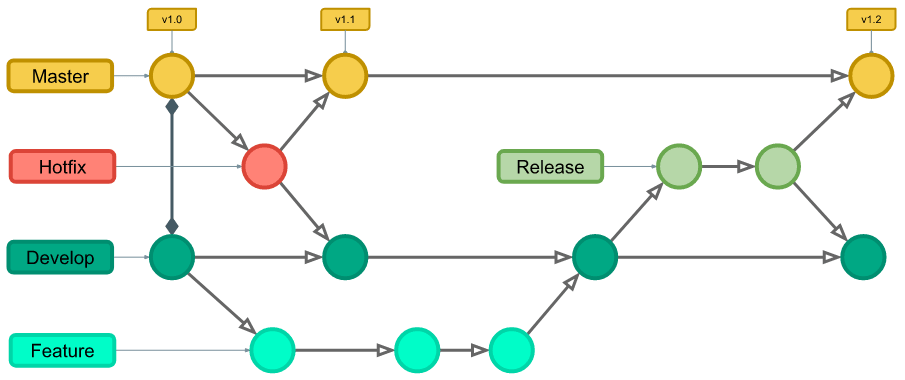
\includegraphics[width=1.0\textwidth]{figures/git_tree.png}
    \caption{Simple example of Git workflow \cite{git-flow}.}
    \label{fig:git-basic-usage}
\end{figure}

Git itself can take years to master as their are now hundreds of commands to memorise, each with their own hyper-specific purpose. Fortunately, becoming confident and competent in Git only requires memorising a handful of commands. In order of usage, most of these are

\begin{enumerate}
    \item \mintinline{shell}{git clone <url> -b <branch>}, clone branch \texttt{<branch>} from the repository \texttt{<url>}
    \item \mintinline{shell}{git branch <name>}, create a branch with name \texttt{<name>} from the current branch
    \item \mintinline{shell}{git checkout <name>}, switch to the branch \texttt{<name>}
    \item \mintinline{shell}{git add <files>}, command Git to start tracking the files \texttt{<files>}
    \begin{enumerate}
        \item Once files have been added, they are referred to as ``staged''
        \item Wildcards are accepted for \texttt{<files>}, e.g. \mintinline{shell}{git add src/*.py} means add all Python source files in the \texttt{src/} directory
    \end{enumerate}
    \item \mintinline{shell}{git commit}, creates a snapshot of the staged files
    \begin{enumerate}
        \item Will open a text file in Vim to write a short message about the commit changes
        \item Can skip Vim usage via \mintinline{shell}{git commit -m "changes made"}
    \end{enumerate}
    \item \mintinline{shell}{git push}, uploads all new commits in current branch to remote repository
\end{enumerate}

\noindent
Other need-to-know commands include

\begin{enumerate}
    \item \mintinline{shell}{git pull}, updates current working branch with new commits from remote repository
    \item \mintinline{shell}{git branch}, displays all branches in the local repository
    \item \mintinline{shell}{git merge <branch>}, combine the history from branch \texttt{<branch>} into current working branch
    \item \mintinline{shell}{git merge}, combines remote repository into current local branch
    \item \mintinline{shell}{git log}, Display version history for the current branch
    \item \mintinline{shell}{git diff <branch1> <branch2>}, compare differences between two branches
    \item \mintinline{shell}{git status}, displays the current working branch, how many commits the branch is from the master branch, what files have been staged, and what modified files have not been staged
    \item \mintinline{shell}{git revert HEAD}, undos the last commit in the current working branch
    \begin{enumerate}
        \item Note that \texttt{HEAD} refers to the current working branch
    \end{enumerate}
    \item \mintinline{shell}{git reset <commit>}, undoes all commits from \texttt{<commit>} onwards
    \item \mintinline{shell}{git restore --staged <files>}, removes added files from the current branch in the tree
    \item \mintinline{shell}{git rm -f <files>}, both deletes the files \texttt{<files>} on your machine and from Git's tree.
    \begin{enumerate}
        \item If a file was deleted without using \mintinline{shell}{git rm <files>}, Git will complain about missing files
        \item To remove a deleted file from Git's tree, use \mintinline{shell}{git commit -a}
    \end{enumerate}
    \item \mintinline{shell}{git blame <file>}, who changed what in \texttt{<file>} and when
\end{enumerate}

\noindent
It is \textbf{strongly} that readers research Git cheat sheets online, pick one, then use it as a reference.

\subsection{Using Github}

With the rapid increase in internet speeds, working off-site, and the willingness for companies to let their developers to work from home, hosting Git repositories locally has largely become a thing of the past. Instead, dedicated online Git repositories take the burden of server management off organisations so they can focus on development. The three most popluar such services are Github, Bitbucket, and Gitlab. Of these three, Github, owned and maintained by Microsoft, is the most popular, especially for small organisations and personal projects. Regardless, all three use Git as their VCS. The main differences between the three is their business models. Fortunately for CIET, the premium services offered by these three are merely nice to have. Hence, Github shall be used for this project as an abritrary choice.

With an online repository setup, the best practice manner of contributing to a project is a somewhat convoluted process. To prevent the project Git repository from becoming populated with unnecessary commits and branches, contributors never actually commit directly into the project. Instead, contributers must ``fork'' the project, creating a copy of the project on their account. With this fork, the contributor can make their commits without affecting the main project repository. Once the desired changes have been made, a ``pull request'' can be made. These pull requests are requests to merge the modified codebase to the set location, typically the main repository the forked one originates from. When the pull request is made, this notifies the moderators or admins of the main repository. The moderator will then review the pull request by inspecting what has changed. If approved, the pull request becomes a merge so that everyone now benefits from the contributor's changes. Usually, a pull request will result in changes being requested, as it is extremely unlikely that the changes in the pull request will satisfy the moderator's or the repository's pull request standards. Sometimes, the pull request is deleted, as the work required to salvage what good exists is more than redoing the pull request. While convoluted, this process ensures all code is reviewed and held to a necessary standard before being made official.

\begin{figure}[t!]
    \centering
    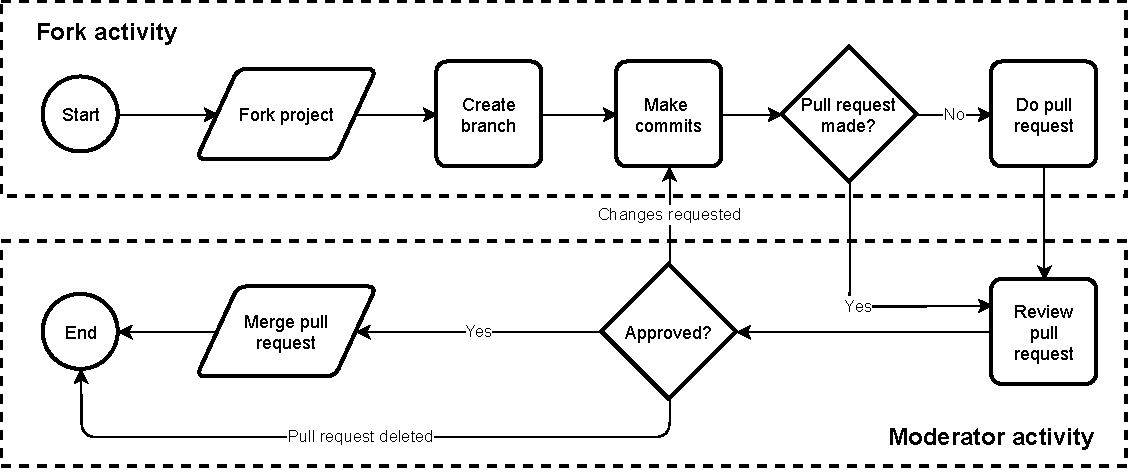
\includegraphics[width=1.0\textwidth]{figures/git_using_forks.pdf}
    \caption{Contributions using Git forks.}
    \label{fig:git-forks}
\end{figure}

\subsection{Recording Library Requirements}

As a matter of practicality, modern software is built using code already written. This can range from using libraries built-in to the language of choice, all the way to using complex frameworks built on so many other layers of libraries, it becomes impossible to fully grasp just how deep and expansive the code reliances are. Regardless of the quantity of external code used, all libraries and frameworks used must be declared.

Python provides a simple manner to explicitly declare what libraries and frameworks are being used. This is achieved through a \mintinline{shell}{requirements.txt} file: a simple text file where each line represents a library or framework, potentially with the accepted versions. Since multiple versions may be compatible with the codebase, there are multiple ways for declaring which versions are acceptable. A double equals (\mintinline{shell}{==}) means only that specific version is accepted, whereas a greater-than-or-equal-to symbol (\mintinline{shell}{>=}) means any version at least as new as the version specified. If a range of versions is accepted, then a comma (\mintinline{shell}{,}) can be used to specify a range. A not equal to symbol (\mintinline{shell}{!=}) means any version except for the one specified (useful if that version has a known bug). Most confusingly, the tilde-equals (\mintinline{shell}{~=}) means a compatible version: so any version matching the same numbers excluding the last number, where the version number must be at least as high as specified. This version is useful for specifying a range without two version numbers. Furthermore, the wildcard \mintinline{shell}{*} is useful for specifying any version matching the start of the specified version. The text below is an example that uses all the version numbering conventions.

\inputminted[linenos=true]{python}{python_examples/requirements_example.txt}

\subsection{Virtual Environments}

While installing libraries and frameworks is a necessity for modern software, it quickly leads to bloat and conflicts. Whenever a library or application is installed, the requirements are also installed. Ergo, even with only a few libraries installed, developers will quickly find their language containing dozens of libraries of various versions. This issue becomes especially problematic when different projects require different versions of the same libraries.

The solution is simple to use but odd to consider. Instead of installing the requirements directly into the installed language, a virtual environment can be made. A virtual environment can be thought of as an isolated instance of the entire programming language for one project. With this isolated instance, libraries and frameworks can be installed without affecting other projects on the same device.

In Python, using virtual environments is handled via the \texttt{virtualenv} package. Once installed with \mintinline{shell}{pip} or \mintinline{shell}{conda}, the virtual environment can be created in the current working directory via

\mint[linenos=false, frame=none]{shell}|python -m venv <name>|

\noindent
where \mintinline{shell}{<name>} is the name of the virtual environment, typically \mintinline{shell}{venv}. A file system will be created with an activiate file. To start the virtual environment, simply type

\mint[linenos=false, frame=none]{shell}|.\<name>\Scripts\activate.bat|

\noindent
on Windows, or

\mint[linenos=false, frame=none]{shell}|source ./<name>/bin/activate|

\noindent
on Unix of MacOS systems. From this point onwards, the virtual environment's Python interpreter will be used, as confirmable by running \mintinline{shell}{which python} in the terminal. Since the virtual environment is made for a specific project, the \mintinline{shell}{requirements.txt} file can be use to install all the required libraries via the command

\mint[linenos=false, frame=none]{shell}|pip install -r requirements.txt|

\noindent
After running the command above, the virtual environment is now ready to run the project files.

\subsection{Further reading}

\begin{itemize}
    \item Git official website: \url{https://git-scm.com/}
    \item Forking a Github repo: \url{https://docs.github.com/en/get-started/quickstart/fork-a-repo}
    \item Github cheatsheet: \url{https://docs.github.com/en/get-started/quickstart/git-cheatsheet}
    \item Python \texttt{requirements.txt} tutorial: \url{https://martin-thoma.com/python-requirements/}
    \item Python virtual environments: \url{https://docs.python.org/3/tutorial/venv.html}
\end{itemize}

\newpage

\section{Coding Standards}

\subsection{Readability and Maintainability}

Any software engineering project will fail before it even starts if coding styles are not established early on. While somewhat subjective, decades of trail and error has revealed multiple key code style principles that greatly assist in the readbility and maintainability of code. These are, in no particular order,

\begin{enumerate}
    \item Identifiers should be short and descriptive.
    \item Class names should be in \mintinline{shell}{PascalCase}.
    \item Constant names should be in \mintinline{shell}{UPPERCASE} with underscores.
    \item Function and variable names should be in \mintinline{shell}{camelCase} or \mintinline{shell}{snake\_case}.
    \item Abbreviations and acrynonyms should only be used when a common convention (e.g. using \mintinline{shell}{num} for \mintinline{shell}{number}), or if obvious based on context.
    \item The naming conventions should be consistent across the entire codebase and documentation.
    \item Short functions are preferred over long functions, even if they lead to more functions.
    \item Global variables must be avoided at all costs.
    \item Whenever it is not obvious as to what a line or block of code is doing or why it is written the way it is, a comment must be provided explaining the why and what.
    \item Comments should only be used for the above situation or providing formal documentation.
    \item Indentation should be used to denote nesting where ever possible.
    \item A complex line of code involving several operations should be split up into shorter simpler lines.
    \item Blank lines should be used to separate blocks of code (e.g. classes and functions).
    \item A single space between operators and operands should be used, excluding around parentheses or before a comma.
    \item A line of code should be no longer than 80 characters.
    \item If a long statement is split across multiple lines of code, the binary operator should start the line; not end it.
    \item \mintinline{python}{import} statements should be at the top of a file, before any other code.
    \begin{enumerate}
        \item From top-to-bottom, the built-in libraries come first, then the third-party ones, then the project libraries.
        \item There should be an empty line inbetween the three different types of libraries.
    \end{enumerate}
    \item Public methods of a class should come before protected ones, then followed by the private ones.
\end{enumerate}

\noindent
Furthermore, Python specific style guide principles can also be established \cite{python-style}:

\begin{itemize}
    \item The datatypes of parameters and return types should be written.
    \item When using the assignment operator (\texttt{=}) to assign a default value, no spaces should be used.
    \item Use four spaces per layer of indentation.
    \item The first parameter of an object method should be \mintinline{python}{self}
    \item The first parameter of a class method should be \mintinline{python}{cls}
    \item \mintinline{python}{... is not ...} is preferred over \mintinline{python}{not ... is ...}
\end{itemize}

\subsection{Documentation comments with docstrings}

Commenting code is a surprisingly controversial subject. On one hand, a lack of comments can lead to vague code that is extremely difficult to understand and maintain. On the other hand, too many comments can lead to code that is annoying to read and maintain, as more text must be read to understand the code and comments may not be updated when the code is changed, leading to misleading documentation. Hence, a balance must be achieved between readability and simplicity.

In Python, docstrings attempt to solve this issue via simple triple quote comments at the start of a class, function, method, or module. A docstring, at a minimum, is comprised of a single line summarises what is being documented \cite{python-docstring}. Additionally, all docstrings may also contain a more detailed description, with a blank line inbetween the summary and description. Functions and methods can also have one line per parameter and return value, detailing their names, datatypes, and purpose. Class docstrings should also have the attributes (i.e. the publicly accessible object variables) and public methods detailed. The example below shows a simple example of an incomplete \mintinline{python}{ComplexNumber} class. Once complete, the \mintinline{python}{__doc__} property or the \mintinline{python}{help()} function can be used to display the docstring without finding and reading the source code.

\inputminted[linenos=true]{python}{python_examples/docstring.py}

\subsection{Sphinx documentation}

Even given detailed and appropriate internal documentation, navigating a source code file system is a time consuming and frustrating process. Often, developers will go around in circles reading the same files over and over again to try and reverse engineer source code. This is an inevitable consequence of complex programs, as code must be organised in a file system to remain organised. However, this organisation will only make inituitive sense to those who made it.

Software engineers have long since known this problem, inventing various documentation generators. Easily the most popular for Python is the Sphinx generator \cite{sphinx}. Sphinx uses the docstrings within source code to automatically generate reStructedText files \cite{rst}, identifiable with the \texttt{.rst} file extension. These reStructedText files can then be used to generate HTML files, allowing for ease of navigating internal documentation with tables of contents, a search engine, and hyperlinks. Furthermore, Sphinx has various HTML themes, both first and third-party, for various aesthetic preferances.

To use Sphinx, a few simple steps must be followed. First, the docstrings must be written for all public constants, classes, methods, and functions. These docstrings must either be writtin in the Sphinx, Google, or NumPy format (the latter two require the \mintinline{python}{napoleon} extension) \cite{sphinx-napolean}. Next, Sphinx must be installed via \mintinline{shell}{pip install sphinx}. After, the command \mintinline{shell}{sphinx-quickstart} can be run to automate most of the \texttt{conf.py} file, which is the settings file for Sphinx when generating documentation.\footnote{It is strongly recommend to run this command in a \texttt{docs/} folder} Then, the reStructedText files can be generated via
\mint[linenos=false, frame=none]{shell}|sphinx-apidoc -o . ../src|

\noindent
Note that the \mintinline{shell}{-o .} tells Sphinx to create the files in the current working directory (e.g. \mintinline{shell}{docs/}), and \mintinline{shell}{../src} tells Sphinx where to look for source code files. Finally, running \mintinline{shell}{make html} tells Sphinx to use the reStructedText files to generate HTML files.

If the docstrings are updated, then the command \mintinline{shell}{make html} can be rerun to update the HTML files. Fortunately, the reStructedText files refer to the docstrings instead of copying them, meaning they do not need to be recreated. For Mac and Linux users, the Makefile program should already be installed \cite{makefile}. For Windows users, Makefile can be installed via installing Chocolatey first, then running \mintinline{shell}{choco install make} \cite{chocolatey}.

\subsection{Further reading}

\begin{itemize}
    \item Official Python code style guide: \url{https://www.python.org/dev/peps/pep-0008/}
    \item Google docstring example: \url{https://sphinxcontrib-napoleon.readthedocs.io/en/latest/example_google.html}
    \item Sphinx official website: \url{https://www.sphinx-doc.org/en/master/}
    \item Idiot's guide to Sphinx: \url{https://samnicholls.net/2016/06/15/how-to-sphinx-readthedocs/}
    \item Official Sphinx HTML themes: \url{https://www.sphinx-doc.org/en/master/usage/theming.html}
    \item Unofficial Sphinx HTML themes: \url{https://sphinx-themes.org/}
    \item Installing Chocolatey: \url{https://chocolatey.org/install}
\end{itemize}

\newpage

\section{Testing Code}

\subsection{Testing tactics}

Testing code has historically gone through several methodologies. At first, code was simply tested by runnning the code and seeing if it works. Such an approach is known as ``exploratory testing'', famous for its ease of use, and notorious for missing bugs. Exploratory testing makes the fundamental mistake in testing: testing is \textit{not} about confirming code works, it is about trying to \textit{break} code. Furthermore, exploratory testing is an extremely repetitive and time-consuming task, leading to testers taking shortcuts and being sloppy. As code must be retested for every update, exploratory testing becomes increasingly inpractical.

To mitigate the issues with exploratory testing, several testing tactics have been developed. First, testing should be planned into test cases: an independent test case that olny checks for one potential failure. With test cases setup, the entire codebase can be thoroughly investigated, diagnosing faults to exact lines of code. Additionally, it is important to note that roughly 80\% of bugs are located in roughly 20\% of the code. With this in mind, writing test cases is a matter of prioritising where bugs typically appear, particularly boundary value analysis (BVA) and equivelance partitioning. Lastly, the error handling of a program must be tested, not just the successful outputs. With these principles in mind, testing can thoroughly investigate the stability of a program with minimal test cases.

\subsection{Historical automated testing using asserts}

Even with the minimisation of test cases, manually testing the code every time it changes is extremely time consuming. Hence, programmers created the \mintinline{python}{assert} statement, allowing for code to be checked automatically. The \mintinline{python}{assert} statement is a simple function that takes in a Boolean value and checks if it is true or false. If true, nothing happens. If false, the \mintinline{python}{assert} function attempts to crash the program with an error messaging stating the assert failed, with a line number and the Boolean expression. In older languages like C, the \mintinline{c}{assert()} function will always crash the program, completely stopping all other subsequent \mintinline{c}{assert()} statements from being checked. Additionally, inserting the \mintinline{c}{assert()} into the source code means they will always be executed every time the program runs, slowing the program down. Python has a slightly more advanced usage form of the \mintinline{python}{assert} statement, allowing for a default error message and, more importantly, throws a catchable \mintinline{python}{AssertionError}, meaning the error can be processed without crashing the entire program, as shown below \cite{python-assert}:

\inputminted[linenos=true]{python}{python_examples/assert_example.py}

While simple, \mintinline{python}{assert} statements are very tedious to work with. This is primarily due to the lack of automated driver code to run the test cases. Instead, the tester must write their own driver code, usually in the form of a \mintinline{python}{main()} function that runs each test case. For each test case, it is possible that the function could raise an error, meaning the driver code must be able to catch errors and process them without crashing the test script, as the subsequent test cases must run. Furthermore, when expecting the same output for different input values, the test cases either become adundant with repetitive code or complex with nested error handling. Lastly, each test case is executed one-by-one, leading to slow test scripts once the test cases become numerous. Fixing this involves complex multiprocessing code, making test scripts difficult to write, maintain, and read.

\subsection{Modern automated testing using \texttt{pytest}}

Multiple frameworks exist for Python to make test scripts smarter, thorough, and easy to use. Of these frameworks, \mintinline{python}{pytest} has proven the simplest and easiest to use without sacrificing test thoroughness \cite{pytest}. By simply overriding Python's \mintinline{python}{assert} statement, \mintinline{python}{pytest} allows developers to write simple code in the form of functions, at least one per test case. Below is a simple script writtin using \mintinline{python}{pytest} framework:

\inputminted{python}{python_examples/pytest_simple.py}

\noindent
Note that every function starts with \mintinline{python}{test_} in their name. This is required for \mintinline{python}{pytest} to recognise the function as a test case that needs to be run. To run the test script, type \mintinline{shell}{pytest <filename>} in the shell. For the example above, the output will be 

\inputminted[linenos=false, frame=none]{shell}{python_examples/pytest_simple_output.txt}

Additionally, \mintinline{python}{pytest} also has several advanced features to allow for smarter design of test scripts. If the exact same input data is used for multiple test cases, a fixture can be used.

\inputminted{python}{python_examples/pytest_fixture.py}

\noindent
Similarly, if multiple sets of data need to be tested against the same test, a parameterised test can be used:

\inputminted{python}{python_examples/pytest_parameterize.py}

\noindent
Lastly, \mintinline{python}{pytest} can run test cases in parallel by installing the \mintinline{shell}{pytest-xdist} plugin, then running \mintinline{python}{pytest} with an \texttt{-n} flag, specifying the number of processes to be created. For example,

\mint[linenos=false, frame=none]{shell}{pytest test_script.py -n 6}

\noindent
will run \texttt{test\_script.py}, splitting the test cases across six processes. \texttt{pytest} also supports third-party plugins that add numerous useful features, the ability to skip failed test cases, and categorising test cases so that only one category of test cases gets executed. Hence, this project should use \texttt{pytest} where ever possible.

\subsection{Mocking functions and classes}

When testing code as independent modules, a problem arises: the modules often rely on each other. Hence, testing one module often requires that other modules are bug free and fully implemented. Obviously, these assumptions are not always valid, needing a manner of testing modules in isolation of each other. Such testing is known as ``unit testing'' or ``component testing'' as code is tested in ``units''.

Fortunately, Python already has a mocking library for this exact purpose \cite{python-mock}. Mocking allows test cases to create mock versions of functions and classes. Furthermore, the \mintinline{python}{pytest-mock} extension for \mintinline{python}{pytest} provides simple wrappers for the mocking library \cite{pytest-mock}. Most importantly, functions are mocked by simply using

\vspace{\baselineskip}
\mintinline{python}{mocker.patch(target, return_value=val)}

\vspace{\baselineskip}

\noindent
In it, the \textit{target} function must be specified as a string of the form \mintinline{python}{package.module.function}. Additionally, the return value of the mock can be specified as \mintinline{python}{return_value=val}, in case the code being tested relies on the function returning a specific value. Similarly, objects can be mocked using

\vspace{\baselineskip}
\noindent
\mintinline{python}{mocker.object(target, attribute, return_value=val)}
\vspace{\baselineskip}

\noindent
where \textit{attribute} is the method being mocked. More mock methods can be added by simply using the \mintinline{python}{mocker.object()} multiple times. Extra rigorous test scripts can also use the \mintinline{python}{assert_called()} functions to ensure the mock functions were called the correct number of times with the correct arguments. Lastly, if the code being mocked should raise an exception, the \mintinline{python}{side_effect} attribute can be used. The code below demonstrates the \mintinline{python}{pytest-mock} extension.

\inputminted[]{python}{python_examples/pytest-mock_example.py}

\subsection{Further reading}

\begin{itemize}
    \item Boundary value analysis and equivalence partioning: \url{https://www.guru99.com/equivalence-partitioning-boundary-value-analysis.html}
    \item Python \mintinline{python}{assert} documentation: \url{https://docs.python.org/3/reference/simple_stmts.html#the-assert-statement}
    \item \texttt{pytest} official website: \url{https://docs.pytest.org/en/6.2.x/}
    \item Mocking official docs: \url{https://docs.python.org/3/library/unittest.mock.html#the-patchers}
    \item \texttt{pytest-mock} PyPI page: \url{https://pypi.org/project/pytest-mock/}
    \item Excellent \texttt{pytest-mock} tutorial: \url{https://changhsinlee.com/pytest-mock/}
\end{itemize}

\newpage

\printbibliography

\end{document}